% Copyright © 2012-2014 Martin Ueding <dev@martin-ueding.de>

% This is my general purpose LaTeX header file for writing German documents.
% Ideally, you include this using a simple ``% Copyright © 2012-2014 Martin Ueding <dev@martin-ueding.de>

% This is my general purpose LaTeX header file for writing German documents.
% Ideally, you include this using a simple ``% Copyright © 2012-2014 Martin Ueding <dev@martin-ueding.de>

% This is my general purpose LaTeX header file for writing German documents.
% Ideally, you include this using a simple ``\input{header.tex}`` in your main
% document and start with ``\title`` and ``\begin{document}`` afterwards.

% If you need to add additional packages, I recommend not doing this in this
% file, but in your main document. That way, you can just drop in a new
% ``header.tex`` and get all the new commands without having to merge manually.

% Since this file encorporates a CC-BY-SA fragment, this whole files is
% licensed under the CC-BY-SA license.

\documentclass[11pt, ngerman, fleqn, DIV=15, headinclude, BCOR=2cm]{scrreprt}

\usepackage{graphicx}

\setkomafont{caption}{\sffamily}
\setkomafont{captionlabel}{\usekomafont{caption}}

%%%%%%%%%%%%%%%%%%%%%%%%%%%%%%%%%%%%%%%%%%%%%%%%%%%%%%%%%%%%%%%%%%%%%%%%%%%%%%%
%                                Locale, date                                 %
%%%%%%%%%%%%%%%%%%%%%%%%%%%%%%%%%%%%%%%%%%%%%%%%%%%%%%%%%%%%%%%%%%%%%%%%%%%%%%%

\usepackage{babel}
\usepackage[iso]{isodate}

%%%%%%%%%%%%%%%%%%%%%%%%%%%%%%%%%%%%%%%%%%%%%%%%%%%%%%%%%%%%%%%%%%%%%%%%%%%%%%%
%                          Margins and other spacing                          %
%%%%%%%%%%%%%%%%%%%%%%%%%%%%%%%%%%%%%%%%%%%%%%%%%%%%%%%%%%%%%%%%%%%%%%%%%%%%%%%

\usepackage[parfill]{parskip}
\usepackage{setspace}
\usepackage[activate]{microtype}

\setlength{\columnsep}{2cm}

%%%%%%%%%%%%%%%%%%%%%%%%%%%%%%%%%%%%%%%%%%%%%%%%%%%%%%%%%%%%%%%%%%%%%%%%%%%%%%%
%                                    Color                                    %
%%%%%%%%%%%%%%%%%%%%%%%%%%%%%%%%%%%%%%%%%%%%%%%%%%%%%%%%%%%%%%%%%%%%%%%%%%%%%%%

\usepackage[usenames, dvipsnames]{xcolor}

\colorlet{darkred}{red!70!black}
\colorlet{darkblue}{blue!70!black}
\colorlet{darkgreen}{green!40!black}

%%%%%%%%%%%%%%%%%%%%%%%%%%%%%%%%%%%%%%%%%%%%%%%%%%%%%%%%%%%%%%%%%%%%%%%%%%%%%%%
%                         Font and font like settings                         %
%%%%%%%%%%%%%%%%%%%%%%%%%%%%%%%%%%%%%%%%%%%%%%%%%%%%%%%%%%%%%%%%%%%%%%%%%%%%%%%

% This replaces all fonts with Bitstream Charter, Bitstream Vera Sans and
% Bitstream Vera Mono. Math will be rendered in Charter.
\usepackage[charter, greekuppercase=italicized]{mathdesign}
\usepackage{beramono}
\usepackage{berasans}

% Bold, sans-serif tensors. This fragment is taken from “egreg” from
% http://tex.stackexchange.com/a/82747/8945 and licensed under `CC-BY-SA
% <https://creativecommons.org/licenses/by-sa/3.0/>`_.
\usepackage{bm}
\DeclareMathAlphabet{\mathsfit}{\encodingdefault}{\sfdefault}{m}{sl}
\SetMathAlphabet{\mathsfit}{bold}{\encodingdefault}{\sfdefault}{bx}{sl}
\newcommand{\tens}[1]{\bm{\mathsfit{#1}}}

% Bold vectors.
\renewcommand{\vec}[1]{\boldsymbol{#1}}

%%%%%%%%%%%%%%%%%%%%%%%%%%%%%%%%%%%%%%%%%%%%%%%%%%%%%%%%%%%%%%%%%%%%%%%%%%%%%%%
%                               Input encoding                                %
%%%%%%%%%%%%%%%%%%%%%%%%%%%%%%%%%%%%%%%%%%%%%%%%%%%%%%%%%%%%%%%%%%%%%%%%%%%%%%%

\usepackage[T1]{fontenc}
\usepackage[utf8]{inputenc}

%%%%%%%%%%%%%%%%%%%%%%%%%%%%%%%%%%%%%%%%%%%%%%%%%%%%%%%%%%%%%%%%%%%%%%%%%%%%%%%
%                         Hyperrefs and PDF metadata                          %
%%%%%%%%%%%%%%%%%%%%%%%%%%%%%%%%%%%%%%%%%%%%%%%%%%%%%%%%%%%%%%%%%%%%%%%%%%%%%%%

\usepackage{hyperref}

% This sets the author in the properties of the PDF as well. If you want to
% change it, just override it with another ``\hypersetup`` call.
\hypersetup{
    breaklinks=false,
    citecolor=darkgreen,
    colorlinks=true,
    linkcolor=darkblue,
    menucolor=black,
    pdfauthor={Martin Ueding},
    urlcolor=darkblue,
}

%%%%%%%%%%%%%%%%%%%%%%%%%%%%%%%%%%%%%%%%%%%%%%%%%%%%%%%%%%%%%%%%%%%%%%%%%%%%%%%
%                               Math Operators                                %
%%%%%%%%%%%%%%%%%%%%%%%%%%%%%%%%%%%%%%%%%%%%%%%%%%%%%%%%%%%%%%%%%%%%%%%%%%%%%%%

% AMS environments like ``align`` and theorems like ``proof``.
\usepackage{amsmath}
\usepackage{amsthm}

% Common math constructs like partial derivatives.
\usepackage{commath}

% Physical units.
\usepackage[output-decimal-marker={,}]{siunitx}

% Since I use mathdesign with italic uppercase greek characters, the Ohm unit will be displayed with an italic Ω by default. Units have to be roman, so this forces it the right way.
\DeclareSIUnit{\ohm}{$\Omegaup$}
\DeclareSIUnit{\division}{DIV}
\DeclareSIUnit{\voltss}{$\mathrm{V_{SS}}$}

% Word like operators.
\DeclareMathOperator{\acosh}{arcosh}
\DeclareMathOperator{\arcosh}{arcosh}
\DeclareMathOperator{\arcsinh}{arsinh}
\DeclareMathOperator{\arsinh}{arsinh}
\DeclareMathOperator{\asinh}{arsinh}
\DeclareMathOperator{\card}{card}
\DeclareMathOperator{\csch}{csch}
\DeclareMathOperator{\diam}{diam}
\DeclareMathOperator{\sech}{sech}
\renewcommand{\Im}{\mathop{{}\mathrm{Im}}\nolimits}
\renewcommand{\Re}{\mathop{{}\mathrm{Re}}\nolimits}

% Fourier transform.
\DeclareMathOperator{\fourier}{\ensuremath{\mathcal{F}}}

% Roman versions of “e” and “i” to serve as Euler's number and the imaginary
% constant.
\newcommand{\eup}{\mathrm e}
\newcommand{\iup}{\mathrm i}

% Symbols for the various mathematical fields (natural numbers, integers,
% rational numbers, real numbers, complex numbers).
\newcommand{\C}{\ensuremath{\mathbb C}}
\newcommand{\N}{\ensuremath{\mathbb N}}
\newcommand{\Q}{\ensuremath{\mathbb Q}}
\newcommand{\R}{\ensuremath{\mathbb R}}
\newcommand{\Z}{\ensuremath{\mathbb Z}}

% Shape like operators.
\DeclareMathOperator{\dalambert}{\Box}
\DeclareMathOperator{\laplace}{\bigtriangleup}
\newcommand{\curl}{\vnabla \times}
\newcommand{\divergence}[1]{\inner{\vnabla}{#1}}
\newcommand{\Divergence}[1]{\Inner{\vnabla}{#1}}
\newcommand{\vnabla}{\vec \nabla}

\newcommand{\half}{\frac 12}

% Unit vector (German „Einheitsvektor“).
\newcommand{\ev}{\hat{\vec e}}

% Mathematician's notation for the inner (scalar, dot) product.
\newcommand{\bracket}[1]{\langle #1 \rangle}
\newcommand{\Bracket}[1]{\left\langle #1 \right\rangle}
\newcommand{\inner}[2]{\bracket{#1, #2}}
\newcommand{\Inner}[2]{\Bracket{#1, #2}}

% Placeholders.
\newcommand{\fehlt}{\textcolor{darkred}{Hier fehlen noch Inhalte.}}
\newcommand{\messwert}{\textcolor{blue}{\square}}
\newcommand{\punkte}{\phantom{xxxxx}}

% Separator for equations on a single line.
\newcommand{\eqnsep}{,\quad}

% Quantum Mechanics.
\usepackage{braket}

% Thermodynamic partial derivative.
\newcommand\tdpd[3]{\del{\dpd{#1}{#2}}_{#3}}

%%%%%%%%%%%%%%%%%%%%%%%%%%%%%%%%%%%%%%%%%%%%%%%%%%%%%%%%%%%%%%%%%%%%%%%%%%%%%%%
%                                  Headings                                   %
%%%%%%%%%%%%%%%%%%%%%%%%%%%%%%%%%%%%%%%%%%%%%%%%%%%%%%%%%%%%%%%%%%%%%%%%%%%%%%%

% This will set fancy headings to the top of the page. The page number will be
% accompanied by the total number of pages. That way, you will know if any page
% is missing.
%
% If you do not want this for your document, you can just use
% ``\pagestyle{plain}``.

\usepackage{scrpage2}

\pagestyle{scrheadings}
\automark{section}
\chead{}
\ihead{}
\ohead{\rightmark}
\setheadsepline{.4pt}

%%%%%%%%%%%%%%%%%%%%%%%%%%%%%%%%%%%%%%%%%%%%%%%%%%%%%%%%%%%%%%%%%%%%%%%%%%%%%%%
%                            Bibliography (BibTeX)                            %
%%%%%%%%%%%%%%%%%%%%%%%%%%%%%%%%%%%%%%%%%%%%%%%%%%%%%%%%%%%%%%%%%%%%%%%%%%%%%%%

\newcommand{\bibliographyfile}{../../central-bibtex/Central}

\usepackage[
    backend=bibtex,
    style=alphabetic,
    %isbn=false,
    %pagetracker=false,
    %maxbibnames=50,
    %maxcitenames=2,
    %autocite=inline,
    %block=space,
    %backref=false,
    %backrefstyle=three+,
    %date=short,
    hyperref=true
]{biblatex}

\setlength{\bibitemsep}{.7em}
\setlength{\bibhang}{4ex}

\IfFileExists{\bibliographyfile}{
    \bibliography{\bibliographyfile}
}{}

%%%%%%%%%%%%%%%%%%%%%%%%%%%%%%%%%%%%%%%%%%%%%%%%%%%%%%%%%%%%%%%%%%%%%%%%%%%%%%%
%                                Abbreviations                                %
%%%%%%%%%%%%%%%%%%%%%%%%%%%%%%%%%%%%%%%%%%%%%%%%%%%%%%%%%%%%%%%%%%%%%%%%%%%%%%%

\newcommand{\dhabk}{\mbox{d.\,h.}}

%%%%%%%%%%%%%%%%%%%%%%%%%%%%%%%%%%%%%%%%%%%%%%%%%%%%%%%%%%%%%%%%%%%%%%%%%%%%%%%
%                                  Licences                                   %
%%%%%%%%%%%%%%%%%%%%%%%%%%%%%%%%%%%%%%%%%%%%%%%%%%%%%%%%%%%%%%%%%%%%%%%%%%%%%%%

\usepackage{ccicons}

\newcommand{\ccbysadetext}{%
    \begin{small}
        Dieses Werk bzw. Inhalt steht unter einer
        \href{http://creativecommons.org/licenses/by-sa/3.0/deed.de}{%
            Creative Commons Namensnennung - Weitergabe unter gleichen
        Bedingungen 3.0 Unported Lizenz}.
    \end{small}
}

\newcommand{\ccbysadetitle}{%
    Lizenz: \href{http://creativecommons.org/licenses/by-sa/3.0/deed.de}
    {CC-BY-SA 3.0 \ccbysa}
}

\newcommand\erklaerungFehlerNotation{%
    In dieser Notation bedeutet \num{1.234 +- 0.005}, dass der Wert
    $\num{1.234} \pm \num{0.005}$ ist. Die Ziffern in Klammern sind die
    Fehlerangabe. Um den Fehler zu erhalten, wird diese von rechts über die
    Zahl gelegt, alle anderen Stellen werden auf 0 gesetzt.
}

`` in your main
% document and start with ``\title`` and ``\begin{document}`` afterwards.

% If you need to add additional packages, I recommend not doing this in this
% file, but in your main document. That way, you can just drop in a new
% ``header.tex`` and get all the new commands without having to merge manually.

% Since this file encorporates a CC-BY-SA fragment, this whole files is
% licensed under the CC-BY-SA license.

\documentclass[11pt, ngerman, fleqn, DIV=15, headinclude, BCOR=2cm]{scrreprt}

\usepackage{graphicx}

\setkomafont{caption}{\sffamily}
\setkomafont{captionlabel}{\usekomafont{caption}}

%%%%%%%%%%%%%%%%%%%%%%%%%%%%%%%%%%%%%%%%%%%%%%%%%%%%%%%%%%%%%%%%%%%%%%%%%%%%%%%
%                                Locale, date                                 %
%%%%%%%%%%%%%%%%%%%%%%%%%%%%%%%%%%%%%%%%%%%%%%%%%%%%%%%%%%%%%%%%%%%%%%%%%%%%%%%

\usepackage{babel}
\usepackage[iso]{isodate}

%%%%%%%%%%%%%%%%%%%%%%%%%%%%%%%%%%%%%%%%%%%%%%%%%%%%%%%%%%%%%%%%%%%%%%%%%%%%%%%
%                          Margins and other spacing                          %
%%%%%%%%%%%%%%%%%%%%%%%%%%%%%%%%%%%%%%%%%%%%%%%%%%%%%%%%%%%%%%%%%%%%%%%%%%%%%%%

\usepackage[parfill]{parskip}
\usepackage{setspace}
\usepackage[activate]{microtype}

\setlength{\columnsep}{2cm}

%%%%%%%%%%%%%%%%%%%%%%%%%%%%%%%%%%%%%%%%%%%%%%%%%%%%%%%%%%%%%%%%%%%%%%%%%%%%%%%
%                                    Color                                    %
%%%%%%%%%%%%%%%%%%%%%%%%%%%%%%%%%%%%%%%%%%%%%%%%%%%%%%%%%%%%%%%%%%%%%%%%%%%%%%%

\usepackage[usenames, dvipsnames]{xcolor}

\colorlet{darkred}{red!70!black}
\colorlet{darkblue}{blue!70!black}
\colorlet{darkgreen}{green!40!black}

%%%%%%%%%%%%%%%%%%%%%%%%%%%%%%%%%%%%%%%%%%%%%%%%%%%%%%%%%%%%%%%%%%%%%%%%%%%%%%%
%                         Font and font like settings                         %
%%%%%%%%%%%%%%%%%%%%%%%%%%%%%%%%%%%%%%%%%%%%%%%%%%%%%%%%%%%%%%%%%%%%%%%%%%%%%%%

% This replaces all fonts with Bitstream Charter, Bitstream Vera Sans and
% Bitstream Vera Mono. Math will be rendered in Charter.
\usepackage[charter, greekuppercase=italicized]{mathdesign}
\usepackage{beramono}
\usepackage{berasans}

% Bold, sans-serif tensors. This fragment is taken from “egreg” from
% http://tex.stackexchange.com/a/82747/8945 and licensed under `CC-BY-SA
% <https://creativecommons.org/licenses/by-sa/3.0/>`_.
\usepackage{bm}
\DeclareMathAlphabet{\mathsfit}{\encodingdefault}{\sfdefault}{m}{sl}
\SetMathAlphabet{\mathsfit}{bold}{\encodingdefault}{\sfdefault}{bx}{sl}
\newcommand{\tens}[1]{\bm{\mathsfit{#1}}}

% Bold vectors.
\renewcommand{\vec}[1]{\boldsymbol{#1}}

%%%%%%%%%%%%%%%%%%%%%%%%%%%%%%%%%%%%%%%%%%%%%%%%%%%%%%%%%%%%%%%%%%%%%%%%%%%%%%%
%                               Input encoding                                %
%%%%%%%%%%%%%%%%%%%%%%%%%%%%%%%%%%%%%%%%%%%%%%%%%%%%%%%%%%%%%%%%%%%%%%%%%%%%%%%

\usepackage[T1]{fontenc}
\usepackage[utf8]{inputenc}

%%%%%%%%%%%%%%%%%%%%%%%%%%%%%%%%%%%%%%%%%%%%%%%%%%%%%%%%%%%%%%%%%%%%%%%%%%%%%%%
%                         Hyperrefs and PDF metadata                          %
%%%%%%%%%%%%%%%%%%%%%%%%%%%%%%%%%%%%%%%%%%%%%%%%%%%%%%%%%%%%%%%%%%%%%%%%%%%%%%%

\usepackage{hyperref}

% This sets the author in the properties of the PDF as well. If you want to
% change it, just override it with another ``\hypersetup`` call.
\hypersetup{
    breaklinks=false,
    citecolor=darkgreen,
    colorlinks=true,
    linkcolor=darkblue,
    menucolor=black,
    pdfauthor={Martin Ueding},
    urlcolor=darkblue,
}

%%%%%%%%%%%%%%%%%%%%%%%%%%%%%%%%%%%%%%%%%%%%%%%%%%%%%%%%%%%%%%%%%%%%%%%%%%%%%%%
%                               Math Operators                                %
%%%%%%%%%%%%%%%%%%%%%%%%%%%%%%%%%%%%%%%%%%%%%%%%%%%%%%%%%%%%%%%%%%%%%%%%%%%%%%%

% AMS environments like ``align`` and theorems like ``proof``.
\usepackage{amsmath}
\usepackage{amsthm}

% Common math constructs like partial derivatives.
\usepackage{commath}

% Physical units.
\usepackage[output-decimal-marker={,}]{siunitx}

% Since I use mathdesign with italic uppercase greek characters, the Ohm unit will be displayed with an italic Ω by default. Units have to be roman, so this forces it the right way.
\DeclareSIUnit{\ohm}{$\Omegaup$}
\DeclareSIUnit{\division}{DIV}
\DeclareSIUnit{\voltss}{$\mathrm{V_{SS}}$}

% Word like operators.
\DeclareMathOperator{\acosh}{arcosh}
\DeclareMathOperator{\arcosh}{arcosh}
\DeclareMathOperator{\arcsinh}{arsinh}
\DeclareMathOperator{\arsinh}{arsinh}
\DeclareMathOperator{\asinh}{arsinh}
\DeclareMathOperator{\card}{card}
\DeclareMathOperator{\csch}{csch}
\DeclareMathOperator{\diam}{diam}
\DeclareMathOperator{\sech}{sech}
\renewcommand{\Im}{\mathop{{}\mathrm{Im}}\nolimits}
\renewcommand{\Re}{\mathop{{}\mathrm{Re}}\nolimits}

% Fourier transform.
\DeclareMathOperator{\fourier}{\ensuremath{\mathcal{F}}}

% Roman versions of “e” and “i” to serve as Euler's number and the imaginary
% constant.
\newcommand{\eup}{\mathrm e}
\newcommand{\iup}{\mathrm i}

% Symbols for the various mathematical fields (natural numbers, integers,
% rational numbers, real numbers, complex numbers).
\newcommand{\C}{\ensuremath{\mathbb C}}
\newcommand{\N}{\ensuremath{\mathbb N}}
\newcommand{\Q}{\ensuremath{\mathbb Q}}
\newcommand{\R}{\ensuremath{\mathbb R}}
\newcommand{\Z}{\ensuremath{\mathbb Z}}

% Shape like operators.
\DeclareMathOperator{\dalambert}{\Box}
\DeclareMathOperator{\laplace}{\bigtriangleup}
\newcommand{\curl}{\vnabla \times}
\newcommand{\divergence}[1]{\inner{\vnabla}{#1}}
\newcommand{\Divergence}[1]{\Inner{\vnabla}{#1}}
\newcommand{\vnabla}{\vec \nabla}

\newcommand{\half}{\frac 12}

% Unit vector (German „Einheitsvektor“).
\newcommand{\ev}{\hat{\vec e}}

% Mathematician's notation for the inner (scalar, dot) product.
\newcommand{\bracket}[1]{\langle #1 \rangle}
\newcommand{\Bracket}[1]{\left\langle #1 \right\rangle}
\newcommand{\inner}[2]{\bracket{#1, #2}}
\newcommand{\Inner}[2]{\Bracket{#1, #2}}

% Placeholders.
\newcommand{\fehlt}{\textcolor{darkred}{Hier fehlen noch Inhalte.}}
\newcommand{\messwert}{\textcolor{blue}{\square}}
\newcommand{\punkte}{\phantom{xxxxx}}

% Separator for equations on a single line.
\newcommand{\eqnsep}{,\quad}

% Quantum Mechanics.
\usepackage{braket}

% Thermodynamic partial derivative.
\newcommand\tdpd[3]{\del{\dpd{#1}{#2}}_{#3}}

%%%%%%%%%%%%%%%%%%%%%%%%%%%%%%%%%%%%%%%%%%%%%%%%%%%%%%%%%%%%%%%%%%%%%%%%%%%%%%%
%                                  Headings                                   %
%%%%%%%%%%%%%%%%%%%%%%%%%%%%%%%%%%%%%%%%%%%%%%%%%%%%%%%%%%%%%%%%%%%%%%%%%%%%%%%

% This will set fancy headings to the top of the page. The page number will be
% accompanied by the total number of pages. That way, you will know if any page
% is missing.
%
% If you do not want this for your document, you can just use
% ``\pagestyle{plain}``.

\usepackage{scrpage2}

\pagestyle{scrheadings}
\automark{section}
\chead{}
\ihead{}
\ohead{\rightmark}
\setheadsepline{.4pt}

%%%%%%%%%%%%%%%%%%%%%%%%%%%%%%%%%%%%%%%%%%%%%%%%%%%%%%%%%%%%%%%%%%%%%%%%%%%%%%%
%                            Bibliography (BibTeX)                            %
%%%%%%%%%%%%%%%%%%%%%%%%%%%%%%%%%%%%%%%%%%%%%%%%%%%%%%%%%%%%%%%%%%%%%%%%%%%%%%%

\newcommand{\bibliographyfile}{../../central-bibtex/Central}

\usepackage[
    backend=bibtex,
    style=alphabetic,
    %isbn=false,
    %pagetracker=false,
    %maxbibnames=50,
    %maxcitenames=2,
    %autocite=inline,
    %block=space,
    %backref=false,
    %backrefstyle=three+,
    %date=short,
    hyperref=true
]{biblatex}

\setlength{\bibitemsep}{.7em}
\setlength{\bibhang}{4ex}

\IfFileExists{\bibliographyfile}{
    \bibliography{\bibliographyfile}
}{}

%%%%%%%%%%%%%%%%%%%%%%%%%%%%%%%%%%%%%%%%%%%%%%%%%%%%%%%%%%%%%%%%%%%%%%%%%%%%%%%
%                                Abbreviations                                %
%%%%%%%%%%%%%%%%%%%%%%%%%%%%%%%%%%%%%%%%%%%%%%%%%%%%%%%%%%%%%%%%%%%%%%%%%%%%%%%

\newcommand{\dhabk}{\mbox{d.\,h.}}

%%%%%%%%%%%%%%%%%%%%%%%%%%%%%%%%%%%%%%%%%%%%%%%%%%%%%%%%%%%%%%%%%%%%%%%%%%%%%%%
%                                  Licences                                   %
%%%%%%%%%%%%%%%%%%%%%%%%%%%%%%%%%%%%%%%%%%%%%%%%%%%%%%%%%%%%%%%%%%%%%%%%%%%%%%%

\usepackage{ccicons}

\newcommand{\ccbysadetext}{%
    \begin{small}
        Dieses Werk bzw. Inhalt steht unter einer
        \href{http://creativecommons.org/licenses/by-sa/3.0/deed.de}{%
            Creative Commons Namensnennung - Weitergabe unter gleichen
        Bedingungen 3.0 Unported Lizenz}.
    \end{small}
}

\newcommand{\ccbysadetitle}{%
    Lizenz: \href{http://creativecommons.org/licenses/by-sa/3.0/deed.de}
    {CC-BY-SA 3.0 \ccbysa}
}

\newcommand\erklaerungFehlerNotation{%
    In dieser Notation bedeutet \num{1.234 +- 0.005}, dass der Wert
    $\num{1.234} \pm \num{0.005}$ ist. Die Ziffern in Klammern sind die
    Fehlerangabe. Um den Fehler zu erhalten, wird diese von rechts über die
    Zahl gelegt, alle anderen Stellen werden auf 0 gesetzt.
}

`` in your main
% document and start with ``\title`` and ``\begin{document}`` afterwards.

% If you need to add additional packages, I recommend not doing this in this
% file, but in your main document. That way, you can just drop in a new
% ``header.tex`` and get all the new commands without having to merge manually.

% Since this file encorporates a CC-BY-SA fragment, this whole files is
% licensed under the CC-BY-SA license.

\documentclass[11pt, ngerman, fleqn, DIV=15, headinclude, BCOR=2cm]{scrreprt}

\usepackage{graphicx}

\setkomafont{caption}{\sffamily}
\setkomafont{captionlabel}{\usekomafont{caption}}

%%%%%%%%%%%%%%%%%%%%%%%%%%%%%%%%%%%%%%%%%%%%%%%%%%%%%%%%%%%%%%%%%%%%%%%%%%%%%%%
%                                Locale, date                                 %
%%%%%%%%%%%%%%%%%%%%%%%%%%%%%%%%%%%%%%%%%%%%%%%%%%%%%%%%%%%%%%%%%%%%%%%%%%%%%%%

\usepackage{babel}
\usepackage[iso]{isodate}

%%%%%%%%%%%%%%%%%%%%%%%%%%%%%%%%%%%%%%%%%%%%%%%%%%%%%%%%%%%%%%%%%%%%%%%%%%%%%%%
%                          Margins and other spacing                          %
%%%%%%%%%%%%%%%%%%%%%%%%%%%%%%%%%%%%%%%%%%%%%%%%%%%%%%%%%%%%%%%%%%%%%%%%%%%%%%%

\usepackage[parfill]{parskip}
\usepackage{setspace}
\usepackage[activate]{microtype}

\setlength{\columnsep}{2cm}

%%%%%%%%%%%%%%%%%%%%%%%%%%%%%%%%%%%%%%%%%%%%%%%%%%%%%%%%%%%%%%%%%%%%%%%%%%%%%%%
%                                    Color                                    %
%%%%%%%%%%%%%%%%%%%%%%%%%%%%%%%%%%%%%%%%%%%%%%%%%%%%%%%%%%%%%%%%%%%%%%%%%%%%%%%

\usepackage[usenames, dvipsnames]{xcolor}

\colorlet{darkred}{red!70!black}
\colorlet{darkblue}{blue!70!black}
\colorlet{darkgreen}{green!40!black}

%%%%%%%%%%%%%%%%%%%%%%%%%%%%%%%%%%%%%%%%%%%%%%%%%%%%%%%%%%%%%%%%%%%%%%%%%%%%%%%
%                         Font and font like settings                         %
%%%%%%%%%%%%%%%%%%%%%%%%%%%%%%%%%%%%%%%%%%%%%%%%%%%%%%%%%%%%%%%%%%%%%%%%%%%%%%%

% This replaces all fonts with Bitstream Charter, Bitstream Vera Sans and
% Bitstream Vera Mono. Math will be rendered in Charter.
\usepackage[charter, greekuppercase=italicized]{mathdesign}
\usepackage{beramono}
\usepackage{berasans}

% Bold, sans-serif tensors. This fragment is taken from “egreg” from
% http://tex.stackexchange.com/a/82747/8945 and licensed under `CC-BY-SA
% <https://creativecommons.org/licenses/by-sa/3.0/>`_.
\usepackage{bm}
\DeclareMathAlphabet{\mathsfit}{\encodingdefault}{\sfdefault}{m}{sl}
\SetMathAlphabet{\mathsfit}{bold}{\encodingdefault}{\sfdefault}{bx}{sl}
\newcommand{\tens}[1]{\bm{\mathsfit{#1}}}

% Bold vectors.
\renewcommand{\vec}[1]{\boldsymbol{#1}}

%%%%%%%%%%%%%%%%%%%%%%%%%%%%%%%%%%%%%%%%%%%%%%%%%%%%%%%%%%%%%%%%%%%%%%%%%%%%%%%
%                               Input encoding                                %
%%%%%%%%%%%%%%%%%%%%%%%%%%%%%%%%%%%%%%%%%%%%%%%%%%%%%%%%%%%%%%%%%%%%%%%%%%%%%%%

\usepackage[T1]{fontenc}
\usepackage[utf8]{inputenc}

%%%%%%%%%%%%%%%%%%%%%%%%%%%%%%%%%%%%%%%%%%%%%%%%%%%%%%%%%%%%%%%%%%%%%%%%%%%%%%%
%                         Hyperrefs and PDF metadata                          %
%%%%%%%%%%%%%%%%%%%%%%%%%%%%%%%%%%%%%%%%%%%%%%%%%%%%%%%%%%%%%%%%%%%%%%%%%%%%%%%

\usepackage{hyperref}

% This sets the author in the properties of the PDF as well. If you want to
% change it, just override it with another ``\hypersetup`` call.
\hypersetup{
    breaklinks=false,
    citecolor=darkgreen,
    colorlinks=true,
    linkcolor=darkblue,
    menucolor=black,
    pdfauthor={Martin Ueding},
    urlcolor=darkblue,
}

%%%%%%%%%%%%%%%%%%%%%%%%%%%%%%%%%%%%%%%%%%%%%%%%%%%%%%%%%%%%%%%%%%%%%%%%%%%%%%%
%                               Math Operators                                %
%%%%%%%%%%%%%%%%%%%%%%%%%%%%%%%%%%%%%%%%%%%%%%%%%%%%%%%%%%%%%%%%%%%%%%%%%%%%%%%

% AMS environments like ``align`` and theorems like ``proof``.
\usepackage{amsmath}
\usepackage{amsthm}

% Common math constructs like partial derivatives.
\usepackage{commath}

% Physical units.
\usepackage[output-decimal-marker={,}]{siunitx}

% Since I use mathdesign with italic uppercase greek characters, the Ohm unit will be displayed with an italic Ω by default. Units have to be roman, so this forces it the right way.
\DeclareSIUnit{\ohm}{$\Omegaup$}
\DeclareSIUnit{\division}{DIV}
\DeclareSIUnit{\voltss}{$\mathrm{V_{SS}}$}

% Word like operators.
\DeclareMathOperator{\acosh}{arcosh}
\DeclareMathOperator{\arcosh}{arcosh}
\DeclareMathOperator{\arcsinh}{arsinh}
\DeclareMathOperator{\arsinh}{arsinh}
\DeclareMathOperator{\asinh}{arsinh}
\DeclareMathOperator{\card}{card}
\DeclareMathOperator{\csch}{csch}
\DeclareMathOperator{\diam}{diam}
\DeclareMathOperator{\sech}{sech}
\renewcommand{\Im}{\mathop{{}\mathrm{Im}}\nolimits}
\renewcommand{\Re}{\mathop{{}\mathrm{Re}}\nolimits}

% Fourier transform.
\DeclareMathOperator{\fourier}{\ensuremath{\mathcal{F}}}

% Roman versions of “e” and “i” to serve as Euler's number and the imaginary
% constant.
\newcommand{\eup}{\mathrm e}
\newcommand{\iup}{\mathrm i}

% Symbols for the various mathematical fields (natural numbers, integers,
% rational numbers, real numbers, complex numbers).
\newcommand{\C}{\ensuremath{\mathbb C}}
\newcommand{\N}{\ensuremath{\mathbb N}}
\newcommand{\Q}{\ensuremath{\mathbb Q}}
\newcommand{\R}{\ensuremath{\mathbb R}}
\newcommand{\Z}{\ensuremath{\mathbb Z}}

% Shape like operators.
\DeclareMathOperator{\dalambert}{\Box}
\DeclareMathOperator{\laplace}{\bigtriangleup}
\newcommand{\curl}{\vnabla \times}
\newcommand{\divergence}[1]{\inner{\vnabla}{#1}}
\newcommand{\Divergence}[1]{\Inner{\vnabla}{#1}}
\newcommand{\vnabla}{\vec \nabla}

\newcommand{\half}{\frac 12}

% Unit vector (German „Einheitsvektor“).
\newcommand{\ev}{\hat{\vec e}}

% Mathematician's notation for the inner (scalar, dot) product.
\newcommand{\bracket}[1]{\langle #1 \rangle}
\newcommand{\Bracket}[1]{\left\langle #1 \right\rangle}
\newcommand{\inner}[2]{\bracket{#1, #2}}
\newcommand{\Inner}[2]{\Bracket{#1, #2}}

% Placeholders.
\newcommand{\fehlt}{\textcolor{darkred}{Hier fehlen noch Inhalte.}}
\newcommand{\messwert}{\textcolor{blue}{\square}}
\newcommand{\punkte}{\phantom{xxxxx}}

% Separator for equations on a single line.
\newcommand{\eqnsep}{,\quad}

% Quantum Mechanics.
\usepackage{braket}

% Thermodynamic partial derivative.
\newcommand\tdpd[3]{\del{\dpd{#1}{#2}}_{#3}}

%%%%%%%%%%%%%%%%%%%%%%%%%%%%%%%%%%%%%%%%%%%%%%%%%%%%%%%%%%%%%%%%%%%%%%%%%%%%%%%
%                                  Headings                                   %
%%%%%%%%%%%%%%%%%%%%%%%%%%%%%%%%%%%%%%%%%%%%%%%%%%%%%%%%%%%%%%%%%%%%%%%%%%%%%%%

% This will set fancy headings to the top of the page. The page number will be
% accompanied by the total number of pages. That way, you will know if any page
% is missing.
%
% If you do not want this for your document, you can just use
% ``\pagestyle{plain}``.

\usepackage{scrpage2}

\pagestyle{scrheadings}
\automark{section}
\chead{}
\ihead{}
\ohead{\rightmark}
\setheadsepline{.4pt}

%%%%%%%%%%%%%%%%%%%%%%%%%%%%%%%%%%%%%%%%%%%%%%%%%%%%%%%%%%%%%%%%%%%%%%%%%%%%%%%
%                            Bibliography (BibTeX)                            %
%%%%%%%%%%%%%%%%%%%%%%%%%%%%%%%%%%%%%%%%%%%%%%%%%%%%%%%%%%%%%%%%%%%%%%%%%%%%%%%

\newcommand{\bibliographyfile}{../../central-bibtex/Central}

\usepackage[
    backend=bibtex,
    style=alphabetic,
    %isbn=false,
    %pagetracker=false,
    %maxbibnames=50,
    %maxcitenames=2,
    %autocite=inline,
    %block=space,
    %backref=false,
    %backrefstyle=three+,
    %date=short,
    hyperref=true
]{biblatex}

\setlength{\bibitemsep}{.7em}
\setlength{\bibhang}{4ex}

\IfFileExists{\bibliographyfile}{
    \bibliography{\bibliographyfile}
}{}

%%%%%%%%%%%%%%%%%%%%%%%%%%%%%%%%%%%%%%%%%%%%%%%%%%%%%%%%%%%%%%%%%%%%%%%%%%%%%%%
%                                Abbreviations                                %
%%%%%%%%%%%%%%%%%%%%%%%%%%%%%%%%%%%%%%%%%%%%%%%%%%%%%%%%%%%%%%%%%%%%%%%%%%%%%%%

\newcommand{\dhabk}{\mbox{d.\,h.}}

%%%%%%%%%%%%%%%%%%%%%%%%%%%%%%%%%%%%%%%%%%%%%%%%%%%%%%%%%%%%%%%%%%%%%%%%%%%%%%%
%                                  Licences                                   %
%%%%%%%%%%%%%%%%%%%%%%%%%%%%%%%%%%%%%%%%%%%%%%%%%%%%%%%%%%%%%%%%%%%%%%%%%%%%%%%

\usepackage{ccicons}

\newcommand{\ccbysadetext}{%
    \begin{small}
        Dieses Werk bzw. Inhalt steht unter einer
        \href{http://creativecommons.org/licenses/by-sa/3.0/deed.de}{%
            Creative Commons Namensnennung - Weitergabe unter gleichen
        Bedingungen 3.0 Unported Lizenz}.
    \end{small}
}

\newcommand{\ccbysadetitle}{%
    Lizenz: \href{http://creativecommons.org/licenses/by-sa/3.0/deed.de}
    {CC-BY-SA 3.0 \ccbysa}
}

\newcommand\erklaerungFehlerNotation{%
    In dieser Notation bedeutet \num{1.234 +- 0.005}, dass der Wert
    $\num{1.234} \pm \num{0.005}$ ist. Die Ziffern in Klammern sind die
    Fehlerangabe. Um den Fehler zu erhalten, wird diese von rechts über die
    Zahl gelegt, alle anderen Stellen werden auf 0 gesetzt.
}



\usepackage{csquotes}

\usepackage{tikz}
\usetikzlibrary{chains}
\usetikzlibrary{shapes.geometric}

\tikzset{device/.style={
                rectangle,
                minimum size=6mm,
                draw=black
            },
            monitor/.style={
                rectangle,
                rounded corners=2mm,
                minimum size=6mm,
                draw=black
            },
        }

\usepackage{pgfplots}
\pgfplotsset{compat=1.5, width=0.8\linewidth, xticklabel style={/pgf/number
format/.cd,use comma}}

\usepgfplotslibrary{external}
\tikzexternalize

\usepackage{booktabs}

\hypersetup{
    pdftitle=
}

\subject{Praktikumsprotokoll}
\title{Nukleare Elektronik und Lebensdauermessung}
\subtitle{Versuch P525 -- Universität Bonn}
\author{
    Martin Ueding \\ \small{\href{mailto:mu@martin-ueding.de}{mu@martin-ueding.de}}
    \and
    Lino Lemmer
}
\publishers{Tutor: Damian-Maria Piontek}

\begin{document}

\maketitle

\tableofcontents

\chapter{Theorie}

\section{Zerfallsschema von ${}^{22}\text{Na}$ und ${}^{133}\text{Ba}$}

Das Moseley'sche Gesetz gibt die Frequenz der charakteristischen
Röntgenstrahlung eines Kerns mit Kernladung $Z$ an:
\parencite[(17.10)]{meschede-gerthsen_24}
\begin{equation}
    \label{eq:moseley}
    E = h \nu = \frac 34 R_\infty c \cdot (Z - 1)^2.
\end{equation}

Nach dem Moseley'schen Gesetz \eqref{eq:moseley} ist die Energie der
$K_\alpha$-Röntgenstrahlung von Barium \SI{<< E_K_alpha_Ba_keV
>>}{\kilo\electronvolt}.

\section{Wechselwirkung von $\gamma$-Strahlung mit Materie}

Trifft $\gamma$-Strahlung auf Materie, finden abhängig von Photonenergie und
Ordnungszahl des Atoms unterschiedliche Effekte statt. Die Abhängigkeit ist in
Abbildung~\ref{fig:wechselwirkung} skizziert.
\begin{figure}
    \centering
    %\includegraphics[.5\textwidth]{../Abbildungen/Wechselwirkung_Demtroeder.pdf}
    \caption{%
        Dominierende Wechselwirkung zwischen $\gamma$-Strahlung und Materie in
        Abhängigkeit von Photonenergie $E_\gamma$ und Ordnungszahl
        $Z$.%\parencite{Demtroeder_4}
    }
    \label{fig:wechselwirkung}
\end{figure}

\subsection{Photoeffekt}

\subsection{Paarbildung}

Zerfällt ein Photon im Coulombfeld eines Atomkerns in ein
Elektron-Positron-Paar, spricht man von einer Paarbildung. Dies kann nur
stattfinden, wenn die Energie des Photons die Ruheenergie der beiden Teilchen
übersteigt, also $E_\gamma > 2m_\mathrm{e}c^2$. Zudem findet es bevorzugt bei
hohen Ordnungszahlen statt.

\subsection{Compton-Streuung}

Als Compton-Streuung bezeichnet man die elastische Streuung von Photonen zum
Beispiel an Elektronen. Die dabei vom Photon an das Elektron übertragene
Energie hängt nur vom Winkel ab und ist Maximal bei einem Streuwinkel von
$\phi = 180^\circ$, also bei einer Rückstreuung, und minimal bei $\phi = 0^\circ$, also wenn
das Elektron nur gestreift wird.

Werden nun viele Photonen mit einer Energie $E_\nu$ gestreut, wie es in einem
Szintillator der Fall ist, ergibt sich ein charakteristisches Bild.
In Abbildung~\ref{fig:Compton} ist idealisiert die Intensität gegen
die an den Szintillator übertragene Energie dargestellt. Das
Compton-Kontinuum entsteht durch die Streuung mit unterschiedlichen Winkeln,
die scharfe Grenze, die so genannte Compton-Kante wird durch den maximalen
Energieübertrag bei $\phi = 180^\circ$ erzeugt. Der Photopeak, oder auch
Full-Energy-Peak bei $E_\nu$ entsteht durch die vollständige Deponierung der
Photonenergie im Szintillator, beispielsweise durch den Photoeffekt.

\begin{figure}
    \centering
    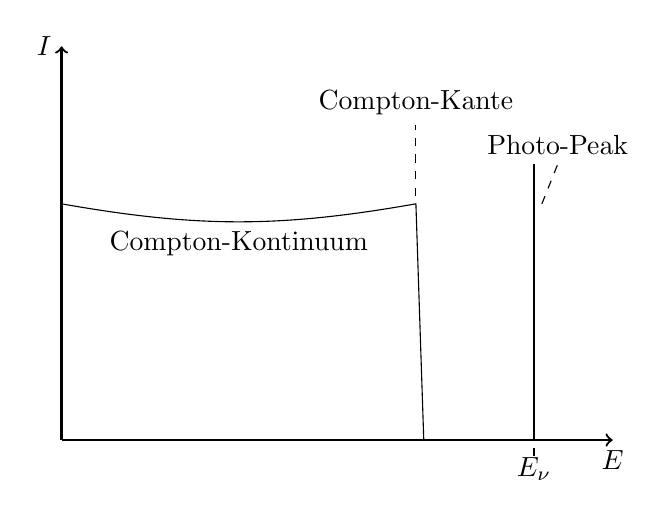
\begin{tikzpicture}
        \draw[thick,->]
        (0,0) -- (0,5) node[left] {$I$}
        ;
        \draw[thick,->]
        (0,0) -- (7,0) node[below] {$E$}
        ;
        \draw
        (6,0) -- (6,3.5)
        ;
        \draw
        (6,-.2) -- (6,-.1) node[below] {$E_\nu$}
        ;
        \draw[bend right=10]
        (0,3) to node[below] {Compton-Kontinuum} (4.5,3) -- (4.6,0)
        ;
        \draw[dashed]
        (4.5,3.1) -- (4.5,4) node[above] {Compton-Kante}
        ;
        \draw[dashed]
        (6.1,3) -- (6.3,3.5) node[above] {Photo-Peak}
        ;
    \end{tikzpicture}
    \caption{%
        Idealisiertes Spektrum der bei Einstrahlung von monochromatischer
        $\gamma$-Strahlung an den Szintillator übertragenen Energie
    }
    \label{fig:Compton}
\end{figure}

\section{Instrumente}

\subsection{Szintillator}

Zur Detektion von $\gamma$-Quanten verwendet man einen Kristall, zum Beispiel
Natriumiodid. Trifft nun ein $\gamma$ auf ein Elektron, wird es angeregt. Bei
der Abregung, die über Zwischenniveaus stattfindet, werden Photonen abgegeben,
welche von einem Photomultiplier eingefangen werden können. Die Intensität des
Lichtblitzes ist dabei proportional zur Energie des ursprünglichen
$\gamma$-Quants.

\subsection{Photomultiplier (PM)}

Will man ein schwaches optisches Signal in eine messbares elektrisches Signal
umwandeln, benötigt man einen Photomultiplier. Ein möglicher Aufbau ist in
Abbildung~\ref{fig:PM} zu sehen. Zwischen Photokathode und Anode liegt eine
Spannung an, die von Dynode zu Dynode abfällt.

Trifft ein Photon auf die Photokathode, löst es, wenn seine Energie die
Austrittsarbeit übersteigt, ein Elektron aus dieser heraus. Durch die angelegte
Spannung wird das Elektron beschleunigt und zum Beispiel durch ein Elektrisches
Feld so abgelenkt, dass es auf die erste Dynode trifft. Hier löst es weitere
Elektronen aus, die zur nächsten Dynode beschleunigt werden. Der Prozess geht
so weiter, bis zum Schluss die Lawinenelektronen auf die Anode treffen und dort
ein messbares elektronisches Signal ergeben.

Da die Anzahl der ausgelösten Elektronen proportional zur Intensität der
eintreffenden Strahlung ist, und da der Photomultiplier linear verstärkt. Ist
das Ausgangssignal proportional zur einfallenden Intensität. Wird ein
Szintillatorsignal verstärkt, ist die Amplitude also proportional zur Energie
der $\gamma$-Strahlung.

\begin{figure}
    \centering
    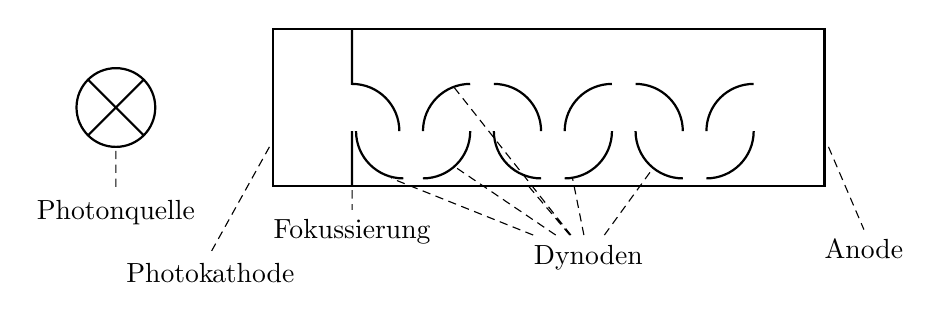
\begin{tikzpicture}
        % Röhre
        \draw[thick] (2,-1) rectangle (9,1);
        % Photonquelle
        \draw[thick]
        (0,0) circle (.5)
        (225:.5) -- (45:.5)
        (135:.5) -- (-45:.5)
        ;
        % Photokathode und Anode
        \draw[thick]
        (2,1) -- (2,-1)
        (9,1) -- (9,-1)
        ;
        % Dynoden
        \draw[thick]
        (3,-.3) -- (3,-1)
        (3,1) -- (3,.3) arc (90:0:.6cm)
        (3.05,-.3) arc (180:270:.6cm)
        (3.9,-.9) arc (270:360:.6cm)
        (3.9,-.3) arc (180:90:.6cm)
        (4.8,.3) arc (90:0:.6cm)
        (4.8,-.3) arc (180:270:.6cm)
        (5.7,-.9) arc (270:360:.6cm)
        (5.7,-.3) arc (180:90:.6cm)
        (6.6,.3) arc (90:0:.6cm)
        (6.6,-.3) arc (180:270:.6cm)
        (7.5,-.9) arc (270:360:.6cm)
        (7.5,-.3) arc (180:90:.6cm)
        ;
        % Beschriftungen PQ, PK, A und Fokussierung
        \draw[densely dashed]
        (0,-.55) -- (0,-1.05) node[below] {Photonquelle}
        (1.95,-.5) -- (1.2,-1.85) node[below] {Photokathode}
        (3,-1.05) -- (3,-1.3) node[below] {Fokussierung}
        (9.05,-.5) -- (9.5,-1.55) node[below] {Anode}
        ;
        % Beschriftung Dynoden
        \node (D) at (6,-1.9) {Dynoden};
        \draw[densely dashed]
        (D) -- (3.5,-.9)
        (D) -- (4.3,-.75)
        (D) -- (4.3,.25)
        (D) -- (5.2,-.95)
        (D) -- (5.8,-.9)
        (D) -- (6.8,-.8)
        ;
    \end{tikzpicture}
    \caption{%
        Möglicher Aufbau eines Photomultipliers
    }
    \label{fig:PM}
\end{figure}

\subsection{Splitter}

\subsection{Verstärker}

Der Verstärker/Operationsverstärker (engl. \emph{amplifier}) ist ein
elektrisches Bauteil, welches die Aufgabe hat ein eingehendes Signal zu
verstärken. Es gibt Strom-, Spannungs- und Ladungsempfindliche Verstärker, je
nach der Art des verstärkten Signales.

%TODO: Funktionsweise

\subsection{Constant Fraction Diskriminator (CFD)}

Ein Diskriminator ist ein Gerät, welches nur anspricht, wenn ein eintreffendes
Signal stärker ist, als ein bestimmter Grenzwert (engl. \emph{threshold}).
Trifft ein solches Signal ein, gibt der Diskriminator ein Standardsignal, zum
Beispiel ein Rechtecksignal aus.

Eine Anwendung des Diskriminators ist das Triggern: Trifft ein Signal ein, wird
ein neues, standardisiertes abgegeben. So ist zum Beispiel der zeitliche
Abstand zwischen zwei eintreffenden Signalen zu messen. Wann genau der
Diskriminator triggert, kommt auf die Art an.

Der CFD triggert, wenn ein bestimmter Anteil der Maximalamplitude erreicht
wird.Dazu wird das einkommende Signal gesplittet, ein Teil wird zeitlich
verzögert, der andere invertiert und um einen Faktor $k$ gedämpft. Anschließend
werden beide Signale wieder addiert. Ein vorher rein positives Signal erhält so
eine Nullstelle, welche durch $k$ bestimmt wird und den Triggerpunkt definiert.

\subsection{Einkanalanalysator (SCA)}

Der SCA ist ein elektrisches Bauteil, welches wie ein Diskriminator eine
Untergrenze hat, unter der Signale blockiert werden. Zusätzlich besitzt er eine
Obergrenze, sodass nur Signale mit einer Amplitude innerhalb eines bestimmten
Bereiches (engl. \emph{window}) betrachtet werden. Er gibt ein logisches Signal
ab, wenn die Amplitude eines einkommendes Signals aus diesem Bereich wieder
unterhalb die Untergrenze fällt.

\subsection{Vielkanalanalysator (MCA)}

Der Vielkanalanalysator sortiert einkommende Signale nach Amplitude. Trifft ein
Signal mit einer bestimmten Amplitude ein, setzt er einen Zähler in einem
bestimmten Kanal hoch. Dadurch zählt der MCA wie häufig die verschiedenen
Amplituden auftauchen. Es entsteht eine Art Histogramm.

\subsection{Koinzidenzeinheit}

Eine Koinzidenzeinheit gibt ein logisches Signal aus, wenn zwei oder mehr
eingehende Signale zeitlich überlappen. Dies kann zum Beispiel realisiert
werden, indem die Amplituden der Signale addiert werden und an einen SCA
übergeben werden, welcher so eingestellt ist, dass er nur anspricht, wenn ein
Signal mit einer Amplitude einkommt, welches der Summe aller eintreffenden
Signale entspricht.

\subsection{Zeit-Impulshöhe-Konverter (TAC)}

Wie der Name schon sagt, konvertiert ein TAC ein Zeitabstand in ein Signal mit
einer zu dieser Zeitdifferenz proportionalen Amplitude. Dies wird erreicht,
indem bei einem Startsignal ein Kondensator mit einem konstanten Strom geladen
wird. Bei einem Stopsignal wird dieser Kondensator über einen Widerstand
entladen. Die Spannung zwischen den Kondensatorplatten ist proportional zur
Zeitdifferenz und die Amplitude proportional zur Spannung. Somit ist die
Amplitude proportional zeitlichen Abstand der Eingangssignale.

%%%%%%%%%%%%%%%%%%%%%%%%%%%%%%%%%%%%%%%%%%%%%%%%%%%%%%%%%%%%%%%%%%%%%%%%%%%%%%%
%                                Durchführung                                %
%%%%%%%%%%%%%%%%%%%%%%%%%%%%%%%%%%%%%%%%%%%%%%%%%%%%%%%%%%%%%%%%%%%%%%%%%%%%%%%

\chapter{Durchführung}

\section{Slow-Koinzidenzkreis einstellen}

Bei der Durchführung am ersten Tag sind wir an einigen Stellen nicht exakt in
der Reihenfolge der Anleitung vorgegangen. Zur besseren Übersicht haben wir
hier die Reihenfolge etwas sortiert. Dabei haben wir auch die Kalibrierung des
linken und rechten Detektors zusammengefasst, um vor allem bei den Abbildungen
einen direkten Vergleich bieten zu können.

\subsection{Slow-Pulse des Photomultipliers kontrollieren}

\begin{figure}[htbp]
    \centering
    \begin{tikzpicture}
        \node[device] (na) {$^{22}\mathrm{Na}$};
        \node[device] (pm) [right=of na] {Photomultiplier};
        \node[monitor] (oszi) [right=of pm] {Oszilloskop};

        % Teilchenaustausch
        \begin{scope}[->, dotted, thick]
            \draw (na) -- (pm);
        \end{scope}

        % Analogsignal
        \begin{scope}[->]
            \draw (pm) -- (oszi);
        \end{scope}

        % Digitalsignal
        \begin{scope}[->, dashdotted]
        \end{scope}
    \end{tikzpicture}
    \caption{%
        Aufbau zum Betrachten des Slow-Signals. Die gepunktete Linie stellt
        Teilchenaustausch (Elektronen, $\gammaup$-Strahlung, …) dar. Die
        durchgezogene Linie ist ein analoges elektrisches Signal. Messgeräte,
        die etwas anzeigen, markieren wir durch die abgerundeten Ecken.
    }
    \label{fig:aufbau:slow}
\end{figure}

Wir betrachten das Slow-Signal des linken Photomultipliers auf dem Oszilloskop
wie in Abbildung~\ref{fig:aufbau:slow} gezeigt. Das Oszillogramm ist in
Abbildung~\ref{fig:slow_signal}, links (Bild 16:26). Dann schauen wir uns das
Slow-Signal des rechten PM auf dem Oszilloskop an, siehe
Abbildung~\ref{fig:slow_signal}, rechts.

\begin{figure}[htbp]
    \centering
    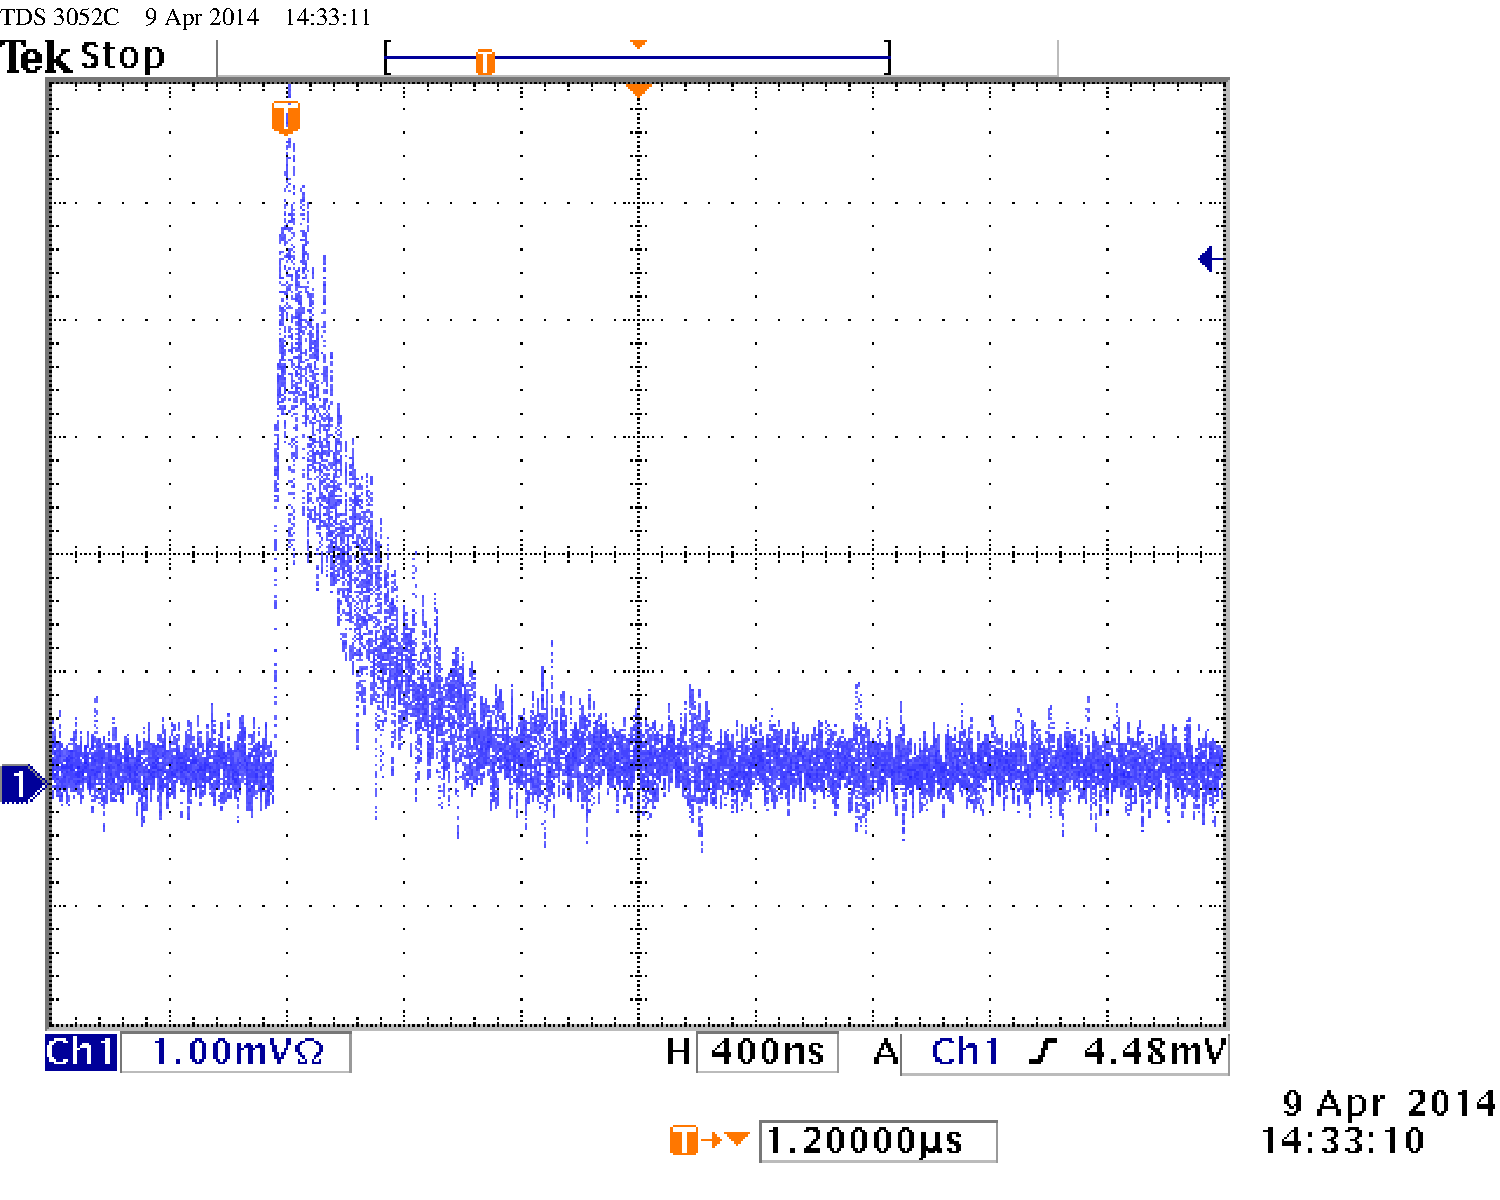
\includegraphics[width=0.49\linewidth]{../Daten/2014-04-09_14-33-east.pdf}
    \hfill
    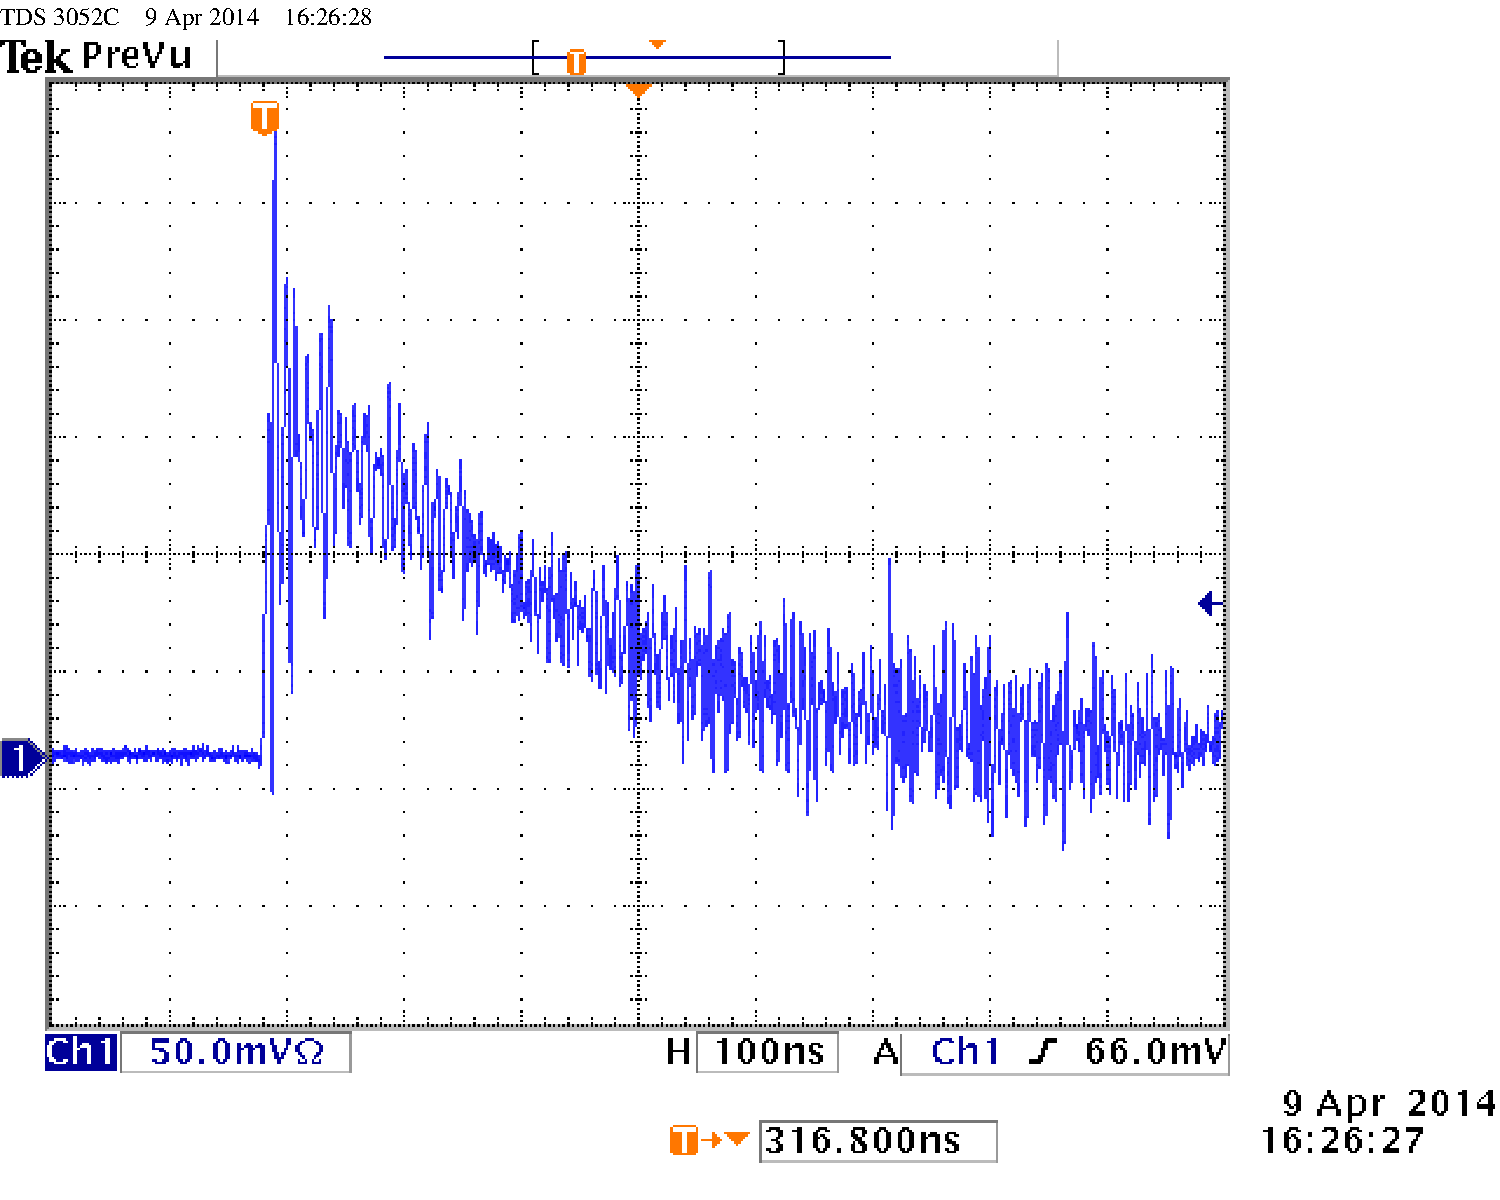
\includegraphics[width=0.49\linewidth]{../Daten/2014-04-09_16-26-east.pdf}
    \caption{%
        Slow-Signale
    }
    \label{fig:slow_signal}
\end{figure}

Danach betrachten wir das Signal nach dem Vorverstärker des linken (Bildzeit
14:58) und rechten (Bildzeit 16:39) Detektors, siehe
Abbildung~\ref{fig:slow_pre_amp}. Der Aufbau ist in
Abbildung~\ref{fig:aufbau:slow_pre} dargestellt.

\begin{figure}[htbp]
    \centering
    \begin{tikzpicture}
        \node[device] (na) {$^{22}\mathrm{Na}$};
        \node[device] (pm) [right=of na] {Photomultiplier};
        \node[device] (preamp) [right=of pm] {Vorverstärker};
        \node[monitor] (oszi) [right=of preamp] {Oszilloskop};

        % Teilchenaustausch
        \begin{scope}[->, dotted, thick]
            \draw (na) -- (pm);
        \end{scope}

        % Analogsignal
        \begin{scope}[->]
            \draw (pm) -- (preamp);
            \draw (preamp) -- (oszi);
        \end{scope}

        % Digitalsignal
        \begin{scope}[->, dashdotted]
        \end{scope}
    \end{tikzpicture}
    \caption{%
        Aufbau zum Betrachten des Slow-Signals nach dem Vorverstärker
    }
    \label{fig:aufbau:slow_pre}
\end{figure}

\begin{figure}[htbp]
    \centering
    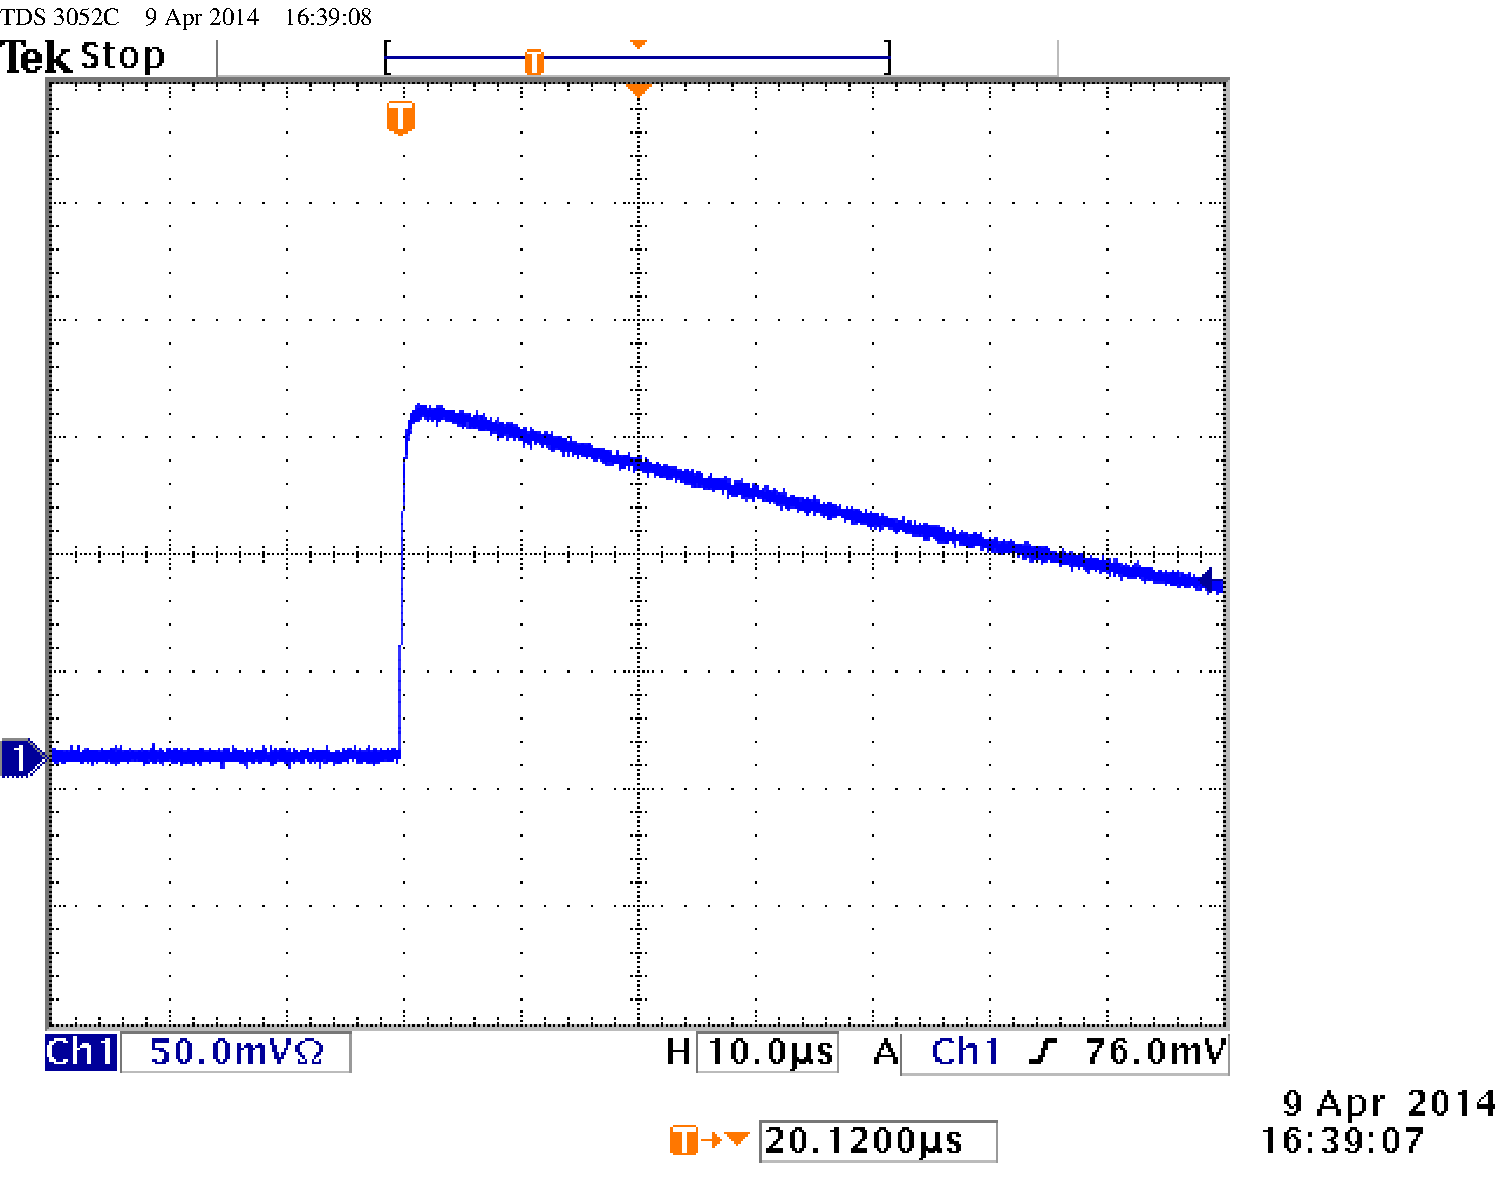
\includegraphics[width=0.49\linewidth]{../Daten/2014-04-09_16-39-east.pdf}
    \hfill
    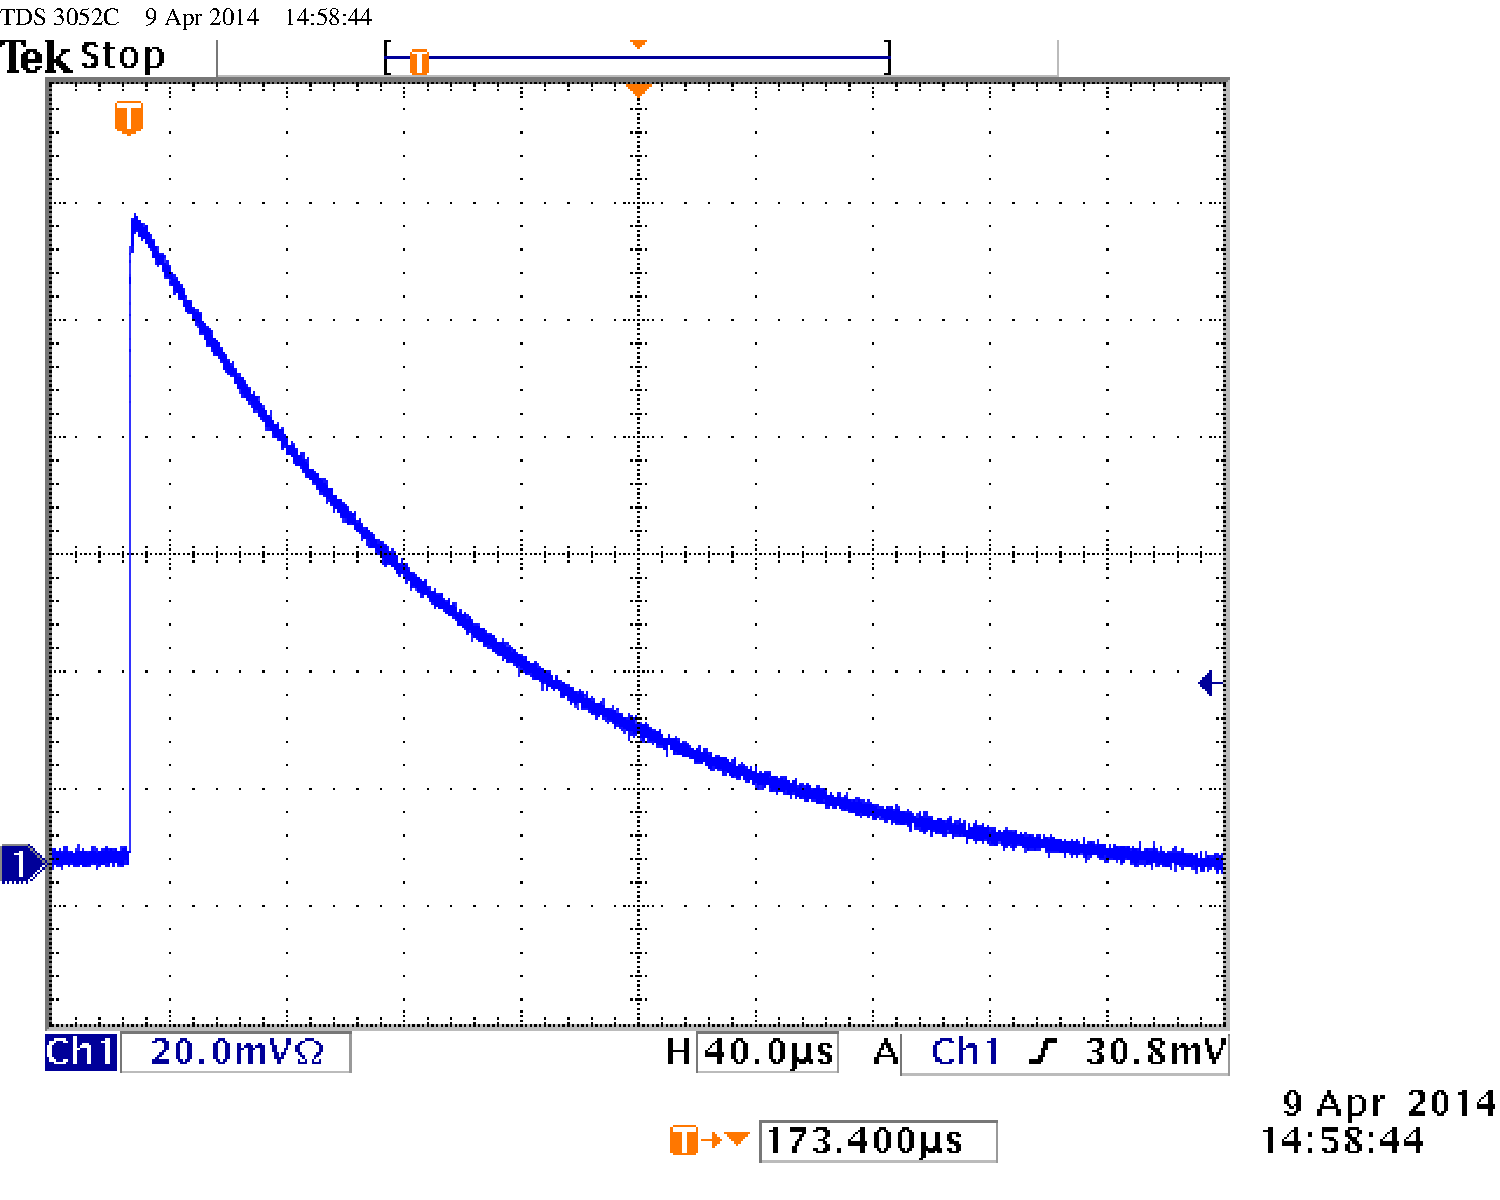
\includegraphics[width=0.49\linewidth]{../Daten/2014-04-09_14-58-east.pdf}
    \caption{%
        Slow-Signal nach dem Vorverstärker
    }
    \label{fig:slow_pre_amp}
\end{figure}

Wir schließen den Hauptverstärker nach dem Vorverstärker an, siehe
Abbildung~\ref{fig:aufbau:slow_amp}. Dessen Ausgang betrachten wir auf dem
Oszilloskop (Bildzeit links 15:03, rechts 16:41), siehe
Abbildung~\ref{fig:slow_amp}.

\begin{figure}[htbp]
    \centering
    \begin{tikzpicture}
        \node[device] (na) {$^{22}\mathrm{Na}$};
        \node[device] (pm) [right=of na] {Photomultiplier};
        \node[device] (preamp) [right=of pm] {Vorverstärker};
        \node[device] (amp) [right=of preamp] {Verstärker};
        \node[monitor] (oszi) [right=of amp] {Oszilloskop};

        % Teilchenaustausch
        \begin{scope}[->, dotted, thick]
            \draw (na) -- (pm);
        \end{scope}

        % Analogsignal
        \begin{scope}[->]
            \draw (pm) -- (preamp);
            \draw (preamp) -- (amp);
            \draw (amp) -- (oszi);
        \end{scope}

        % Digitalsignal
        \begin{scope}[->, dashdotted]
        \end{scope}
    \end{tikzpicture}
    \caption{%
        Aufbau zum Betrachten des Slow-Signals nach dem Hauptverstärker
    }
    \label{fig:aufbau:slow_amp}
\end{figure}

\begin{figure}[htbp]
    \centering
    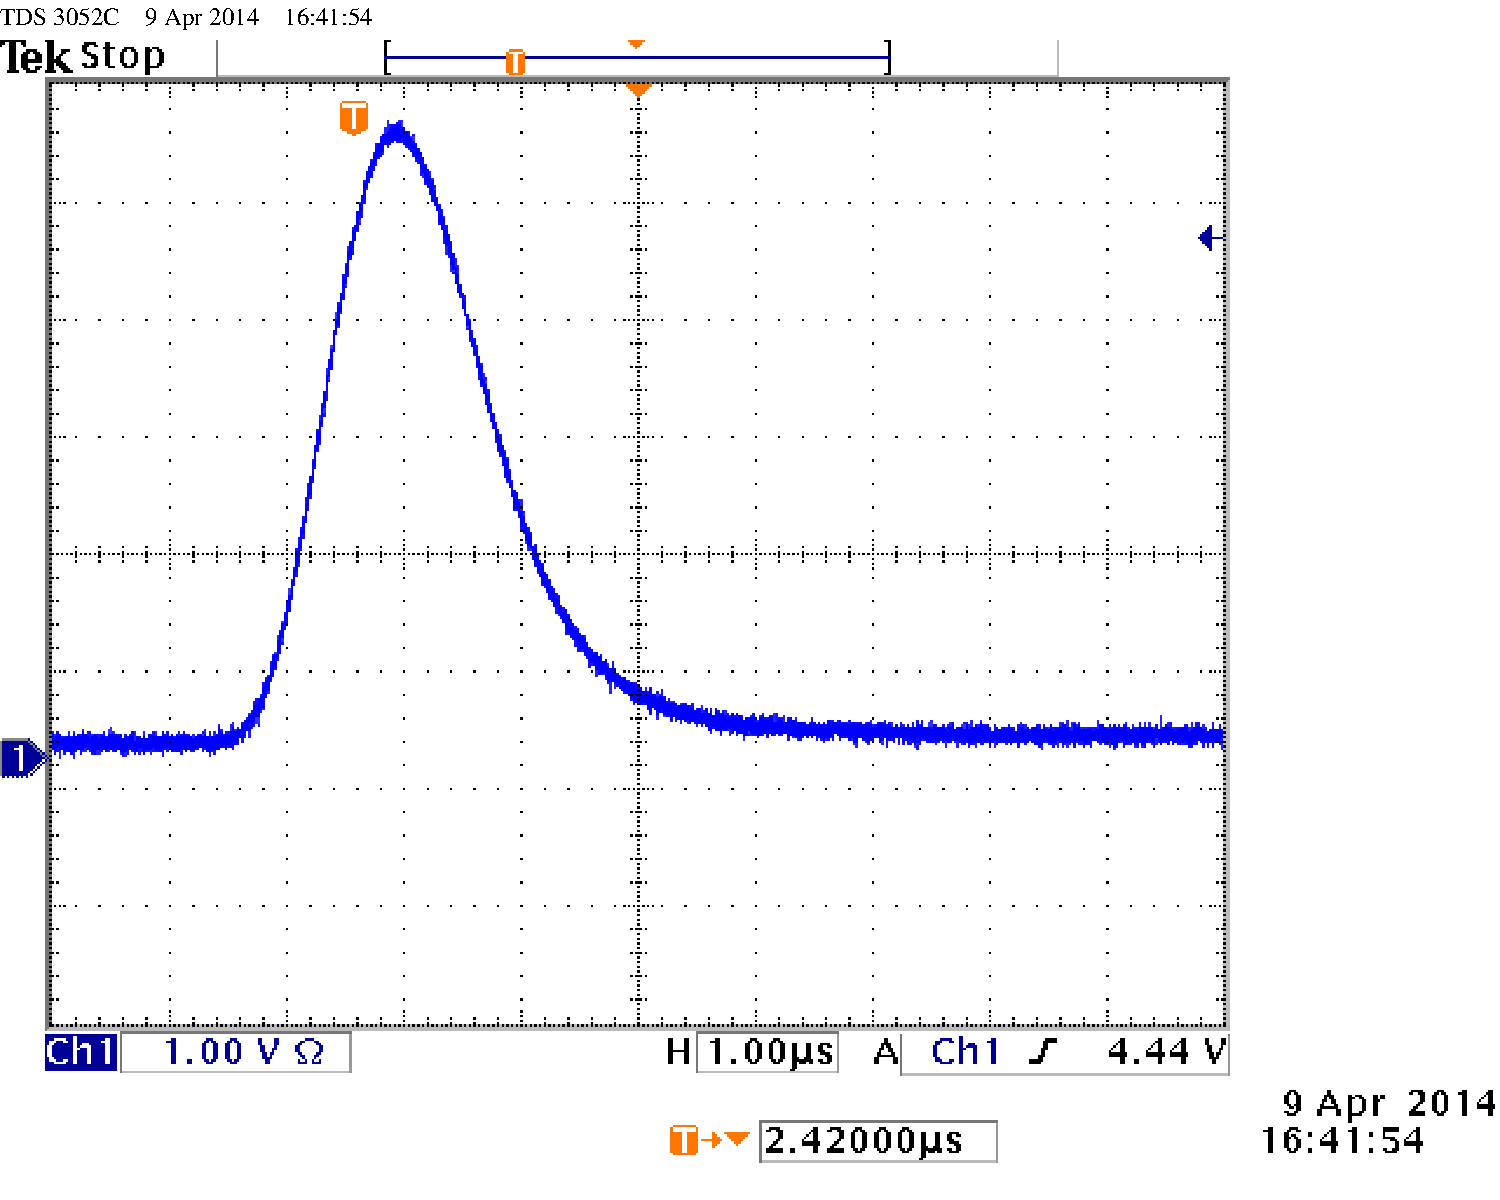
\includegraphics[width=0.49\linewidth]{../Daten/2014-04-09_16-41-east.pdf}
    \hfill
    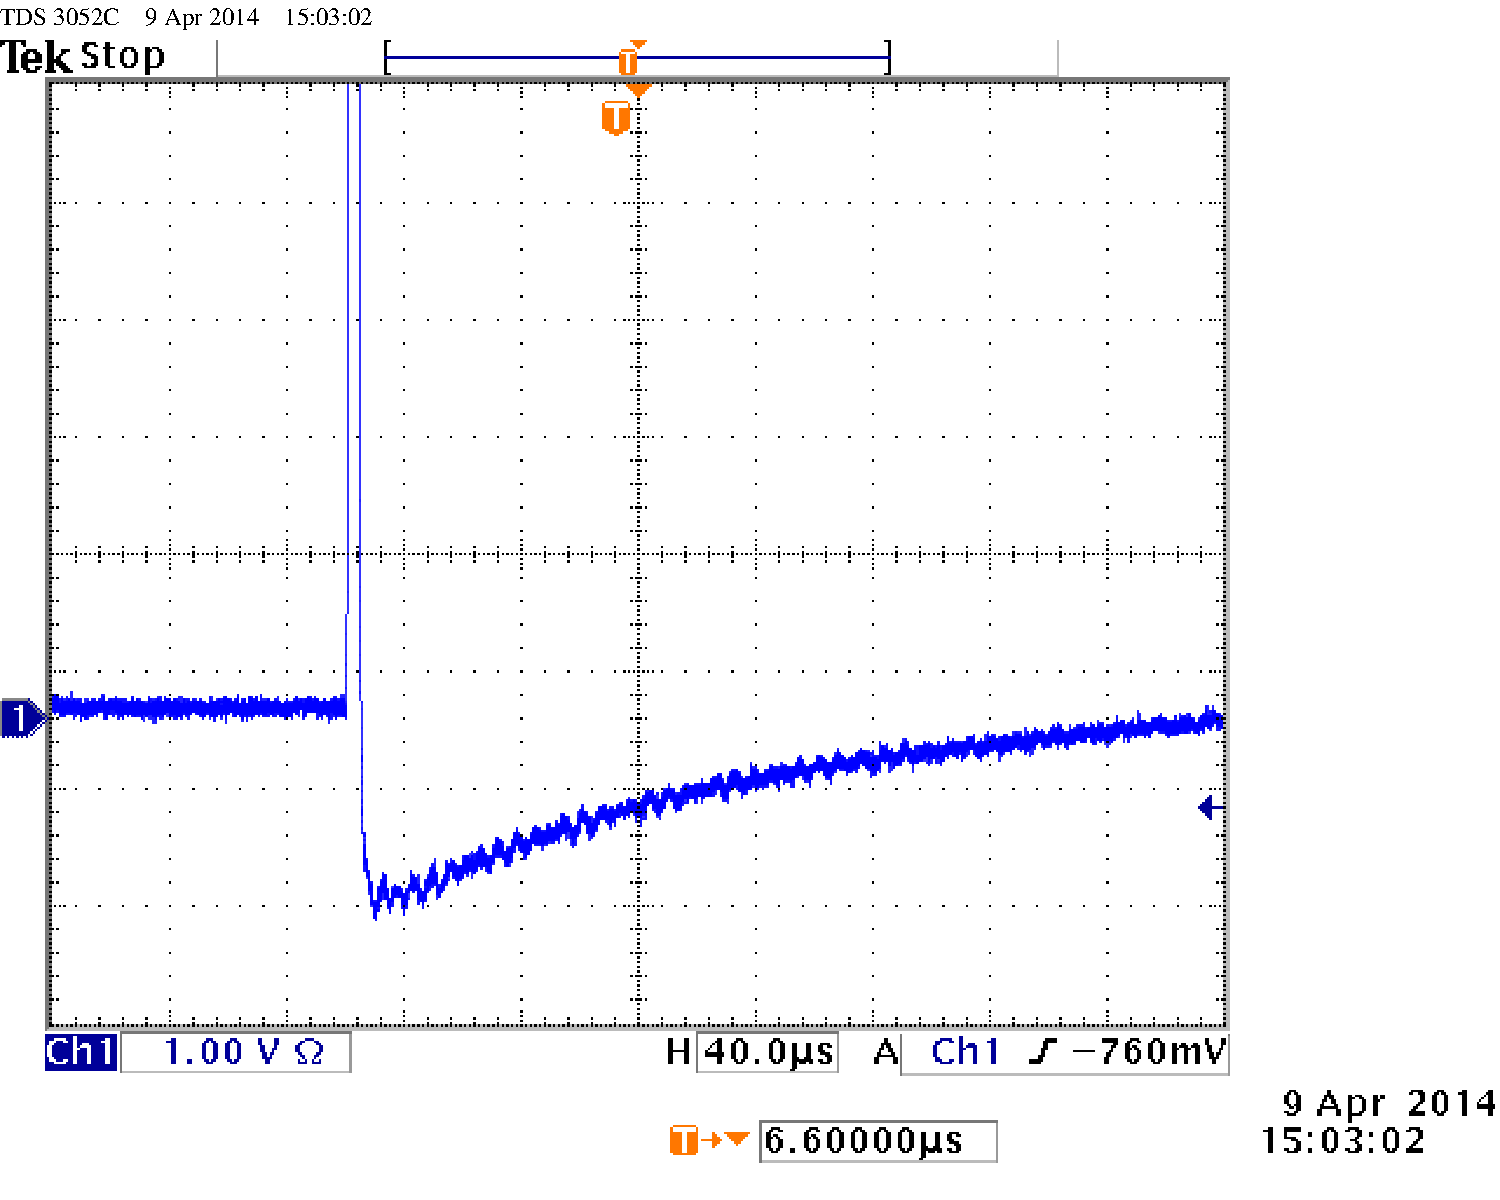
\includegraphics[width=0.49\linewidth]{../Daten/2014-04-09_15-03-east.pdf}
    \caption{%
        Slow-Signal nach dem Verstärker
    }
    \label{fig:slow_amp}
\end{figure}

\subsection{Triggerung mit dem SCA}

Wir schließen den Ausgang des linken Hauptverstärkers an den Splitter an. Der
eine Ausgang geht an das SCA. Der Andere an Delay-Verstärker. Die Ausgänge
beider Geräte betrachten wir mit dem Oszilloskop, siehe
Abbildung~\ref{fig:aufbau:sca_trigger}. Nun versuchen wir, die Verzögerung so
einzustellen, dass das digitale Signal des SCA den Puls vom Verstärker
umschließt. Dies gelingt uns allerdings nicht, weil das digitale Signal zu kurz
ist.

\begin{figure}[htbp]
    \centering
    \begin{tikzpicture}
        \node[device] (na) {$^{22}\mathrm{Na}$};
        \node[device] (pm) [right=of na] {Photomultiplier};
        \node[device] (amp) [right=of pm] {Verstärker};
        \node[device] (split) [right=of amp] {Splitter};
        \node[device] (delay) [right=of split] {Verzögerung};
        \node[device] (sca) [below=of split] {SCA};
        \node[monitor] (oszi) [below=of delay] {Oszilloskop};

        % Teilchenaustausch
        \begin{scope}[->, dotted, thick]
            \draw (na) -- (pm);
        \end{scope}

        % Analogsignal
        \begin{scope}[->]
            \draw (pm) -- (amp);
            \draw (amp) -- (split);
            \draw (split) -- (delay);
            \draw (split) -- (sca);
            \draw (delay) -- (oszi);
        \end{scope}

        % Digitalsignal
        \begin{scope}[->, dashdotted]
            \draw (sca) -- (oszi);
        \end{scope}
    \end{tikzpicture}
    \caption{%
        Aufbau zur Triggerung mit dem SCA. Um Platz zu sparen, fassen wir ab
        hier den Vorverstärker und den Hauptverstärker zu einem Bauteil
        zusammen. Die gestrichpunktete Linie stellt ein digitales Signal dar.
        Das Oszilloskop wird mit dem digitalen Signal getriggert.
    }
    \label{fig:aufbau:sca_trigger}
\end{figure}

Wir regeln den Verstärker auf Faktor 20 herunter. Im Nachleuchten auf dem
Oszilloskop ist eine Amplitude zu erkennen, die besonders häufig vorkommt. Davon
haben wir ein Bild so gespeichert, dass diese Linie auch besonders stark
repräsentiert ist (Bildzeit 15:20), siehe Abbildung~\ref{fig:511}.

\begin{figure}[htbp]
    \centering
    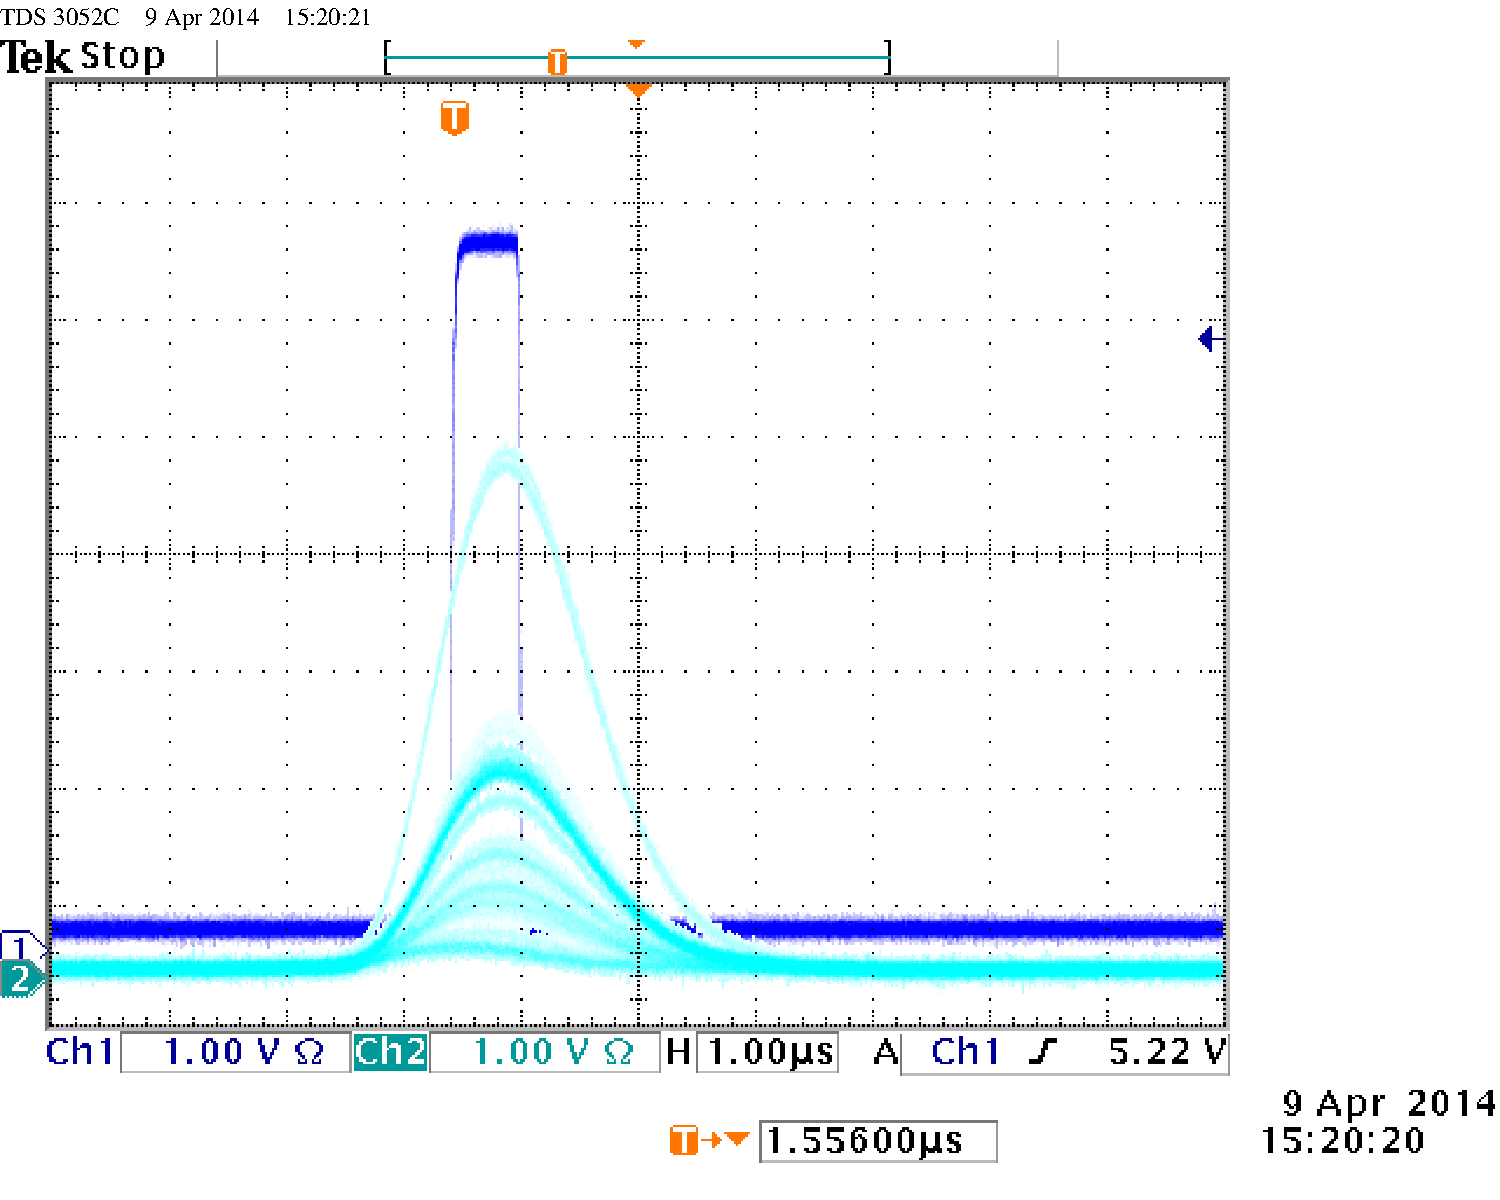
\includegraphics[width=0.49\linewidth]{../Daten/2014-04-09_15-20-east.pdf}
    \caption{%
        Besonders häufig vorkommende Linie im Signal des Verstärkers
    }
    \label{fig:511}
\end{figure}

Zwischen SCA und Oszilloskop schalten wir noch den GDG
(Abbildung~\ref{fig:aufbau:sca_gdg}). Am SCA stellen wir den Delay auf 0. Das
GDG justieren wir so, dass das digitale Signal die Pulse umschließt (Bildzeit
15:27). Am linken Delay-Amp stellen wir eine Verzögerung von
\SI{3.25}{\micro\second} ein. Am GDG stellen wir die Verzögerung aus. Am
Rechten Delay haben wir eine Verzögerung von \SI{3.5}{\micro\second} gewählt.
Das Oszillogramm für den rechten Zweig (Bildzeit 16:47) haben wir in
Abbildung~\ref{fig:sca_umschlossen}

\begin{figure}[htbp]
    \centering
    \begin{tikzpicture}
        \node[device] (na) {$^{22}\mathrm{Na}$};
        \node[device] (pm) [above=of na] {Photomultiplier};
        \node[device] (amp) [right=of pm] {Verstärker};
        \node[device] (split) [right=of amp] {Splitter};
        \node[device] (delay) [right=of split] {Verzögerung};
        \node[device] (sca) [below=of split] {SCA};
        \node[device] (gdg) [right=of sca] {GDG};
        \node[monitor] (oszi) [right=of gdg] {Oszilloskop};

        % Teilchenaustausch
        \begin{scope}[->, dotted, thick]
            \draw (na) -- (pm);
        \end{scope}

        % Analogsignal
        \begin{scope}[->]
            \draw (pm) -- (amp);
            \draw (amp) -- (split);
            \draw (split) -- (delay);
            \draw (split) -- (sca);
            \draw (delay) -- (oszi);
        \end{scope}

        % Digitalsignal
        \begin{scope}[->, dashdotted]
            \draw (sca) -- (gdg);
            \draw (gdg) -- (oszi);
        \end{scope}
    \end{tikzpicture}
    \caption{%
        Aufbau zur Triggerung mit dem SCA und GDG.
    }
    \label{fig:aufbau:sca_gdg}
\end{figure}

\begin{figure}[htbp]
    \centering
    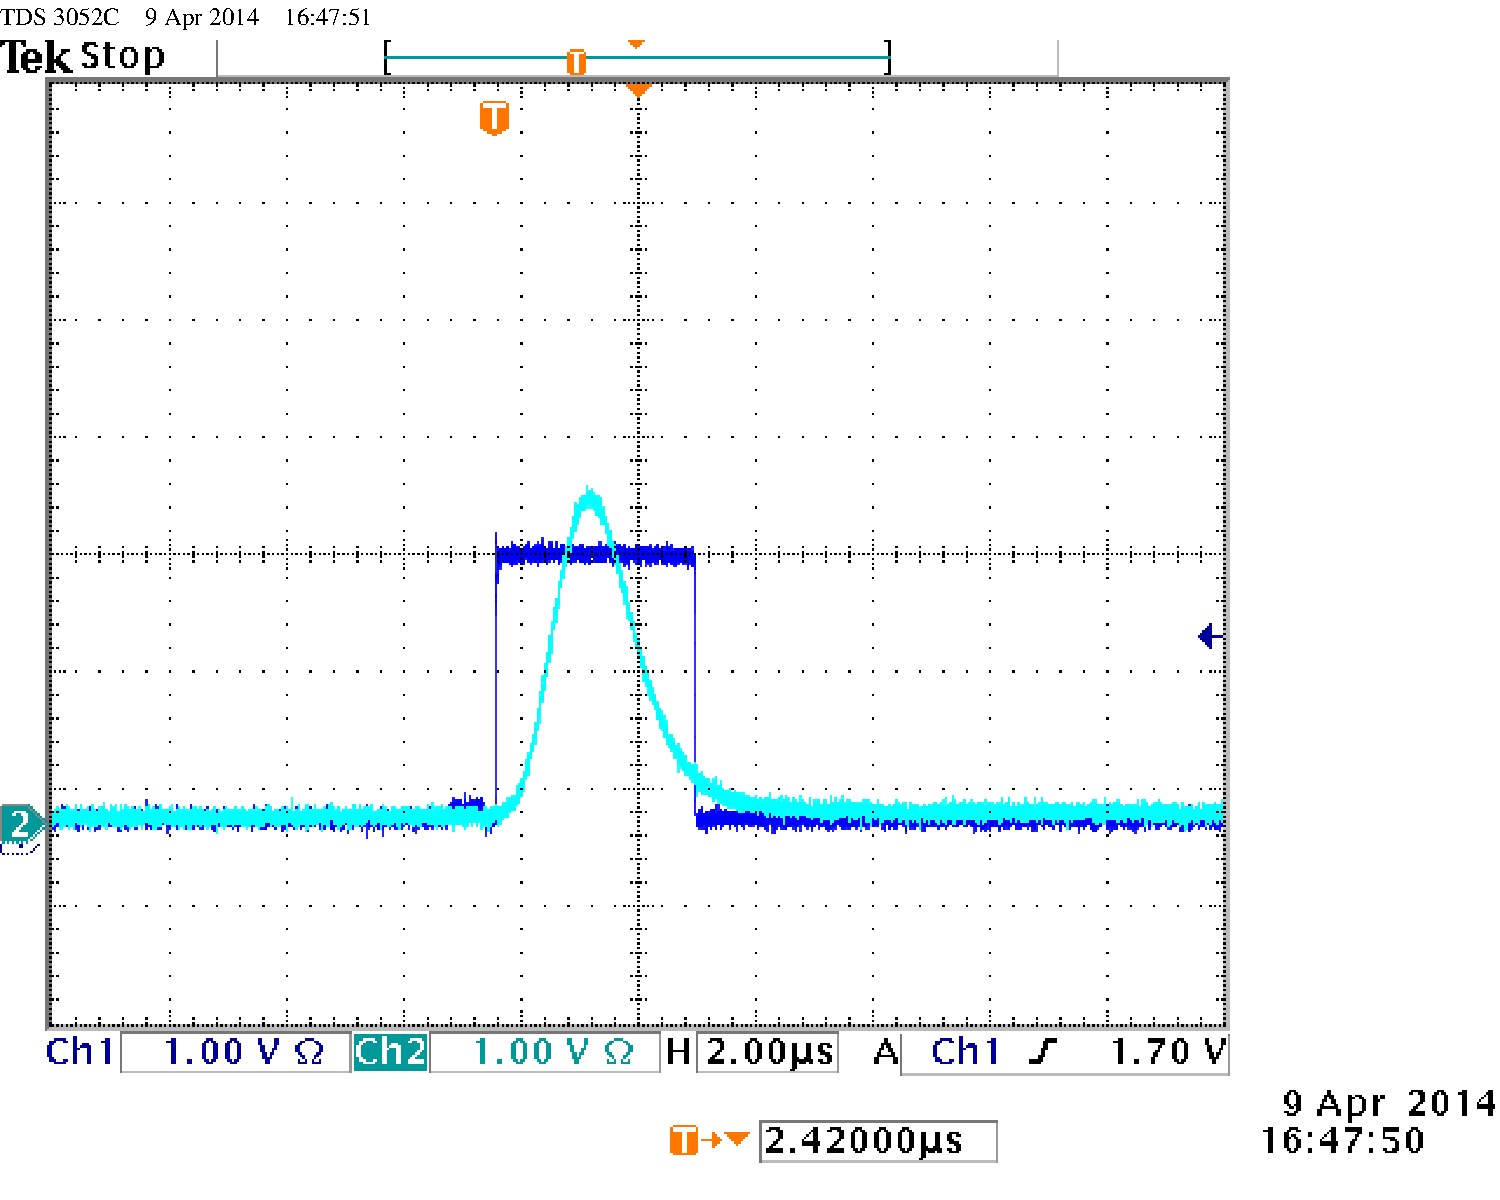
\includegraphics[width=0.49\linewidth]{../Daten/2014-04-09_16-47-east.pdf}
    \caption{%
        Slow-Signal des rechten Detektors nach dem Hauptverstärker im ersten
        Kanal. Das Signal aus dem rechten SCA im zweiten Kanal.
    }
    \label{fig:sca_umschlossen}
\end{figure}

Analog zum vorherigen Teil schließen wir den rechten Hauptverstärker an den
zweiten Splitter an. Die Ausgänge vom Splitter schließen wir an den anderen SCA
sowie an den einen GDG an.

\subsection{Energiespektrum für die ${}^{22}\text{Na}$-Quelle aufnehmen}

Nun ersetzen wir das Oszilloskop durch den MCA und betrachten das Spektrum,
siehe Abbildung~\ref{fig:aufbau:sca_gdg_mca}. Das
Fenster im SCA stellen wir auf die maximale Größe ein (001-Na.txt), siehe
Abbildung~\ref{mca:001_004}.

\begin{figure}[htbp]
    \centering
    \begin{tikzpicture}
        \node[device] (na) {$^{22}\mathrm{Na}$};
        \node[device] (pm) [above=of na] {Photomultiplier};
        \node[device] (amp) [right=of pm] {Verstärker};
        \node[device] (split) [right=of amp] {Splitter};
        \node[device] (delay) [right=of split] {Verzögerung};
        \node[device] (sca) [below=of split] {SCA};
        \node[device] (gdg) [right=of sca] {GDG};
        \node[monitor] (mca) [right=of gdg] {MCA};

        % Teilchenaustausch
        \begin{scope}[->, dotted, thick]
            \draw (na) -- (pm);
        \end{scope}

        % Analogsignal
        \begin{scope}[->]
            \draw (pm) -- (amp);
            \draw (amp) -- (split);
            \draw (split) -- (delay);
            \draw (split) -- (sca);
            \draw (delay) -- (mca);
        \end{scope}

        % Digitalsignal
        \begin{scope}[->, dashdotted]
            \draw (sca) -- (gdg);
            \draw (gdg) -- (mca);
        \end{scope}
    \end{tikzpicture}
    \caption{%
        Aufbau zur Spektrumsaufnahme mit dem SCA und GDG. Das digitale Signal
        wird als Gate im MCA benutzt.
    }
    \label{fig:aufbau:sca_gdg_mca}
\end{figure}

\begin{figure}[htbp]
    \centering
    \begin{tikzpicture}
        \begin{axis}[width=0.45\linewidth, height=0.3\linewidth, xlabel=Kanal, ylabel=Ereignisse, axis lines=left]
            \addplot[black] table {../Daten/004-Na-rechts.txt};
        \end{axis}
    \end{tikzpicture}
    \hfill
    \begin{tikzpicture}
        \begin{axis}[width=0.45\linewidth, height=0.3\linewidth, xlabel=Kanal, ylabel=Ereignisse, axis lines=left]
            \addplot[black] table {../Daten/001-Na.txt};
        \end{axis}
    \end{tikzpicture}
    \caption{Spektrum der Na-Probe im rechten und linken Detektor}
    \label{mca:001_004}
\end{figure}

Damit das Spektrum den ganzen Messbereich des MCA ausfüllt, stellen wir die
Verstärkung des linken Hauptverstärkers auf Faktor 100. Das gleiche stellen für
später auch für den rechten Kreis ein. Beide Spektren sind in
Abbildung~\ref{mca:003_005} dargestellt.

\begin{figure}[htbp]
    \centering
    \begin{tikzpicture}
        \begin{axis}[width=0.45\linewidth, height=0.3\linewidth, xlabel=Kanal, ylabel=Ereignisse, axis lines=left]
            \addplot[black] table {../Daten/005-Na-Zoom.txt};
        \end{axis}
    \end{tikzpicture}
    \hfill
    \begin{tikzpicture}
        \begin{axis}[width=0.45\linewidth, height=0.3\linewidth, xlabel=Kanal, ylabel=Ereignisse, axis lines=left]
            \addplot[black] table {../Daten/003-Na-Spektrum.txt};
        \end{axis}
    \end{tikzpicture}
    \caption{%
        Spektrum der Na-Probe im rechten und linken Detektor mit höherer
        Verstärkung, so dass die \SI{511}{\kilo\electronvolt}-Linie am rechten
        Rand ist
    }
    \label{mca:003_005}
\end{figure}

\subsection{Einkanalfenster für die ${}^{22}\text{Na}$-Quelle einstellen}

Als nächstes justieren wir das
Fenster des linken SCA so, dass nur noch die \SI{511}{\kilo\electronvolt} Linie
wächst. Beim SCA ist als obere Grenze MAX eingestellt, als untere \num{7.31}.
Beim rechten SCA haben wir als untere Grenze \num{6.73} erhalten. Das
resultierende Spektrum ist in Abbildung~\ref{mca:fenster} gezeigt.

\begin{figure}[htbp]
    \centering
    \begin{tikzpicture}
        \begin{axis}[width=0.45\linewidth, height=0.3\linewidth, xlabel=Kanal, ylabel=Ereignisse, axis lines=left]
            \addplot[black] table {../Daten/006-Na-511keV.txt};
        \end{axis}
    \end{tikzpicture}
    \hfill
    \begin{tikzpicture}
        \begin{axis}[width=0.45\linewidth, height=0.3\linewidth, xlabel=Kanal, ylabel=Ereignisse, axis lines=left]
            \addplot[black] table {../Daten/007-Na-SCA-neu.txt};
        \end{axis}
    \end{tikzpicture}
    \caption{%
        Einstellung der SCA Schwellen, so dass nur die
        \SI{511}{\kilo\electronvolt}-Linie wächst.
    }
    \label{mca:fenster}
\end{figure}

Auf dem Oszilloskop sehen wir, dass nur noch eine Pulshöhe zu erkennen ist (Bildzeit
links 17:34, rechts 17:35), siehe Abbildung~\ref{fig:eine_pulshoehe}.

\begin{figure}[htbp]
    \centering
    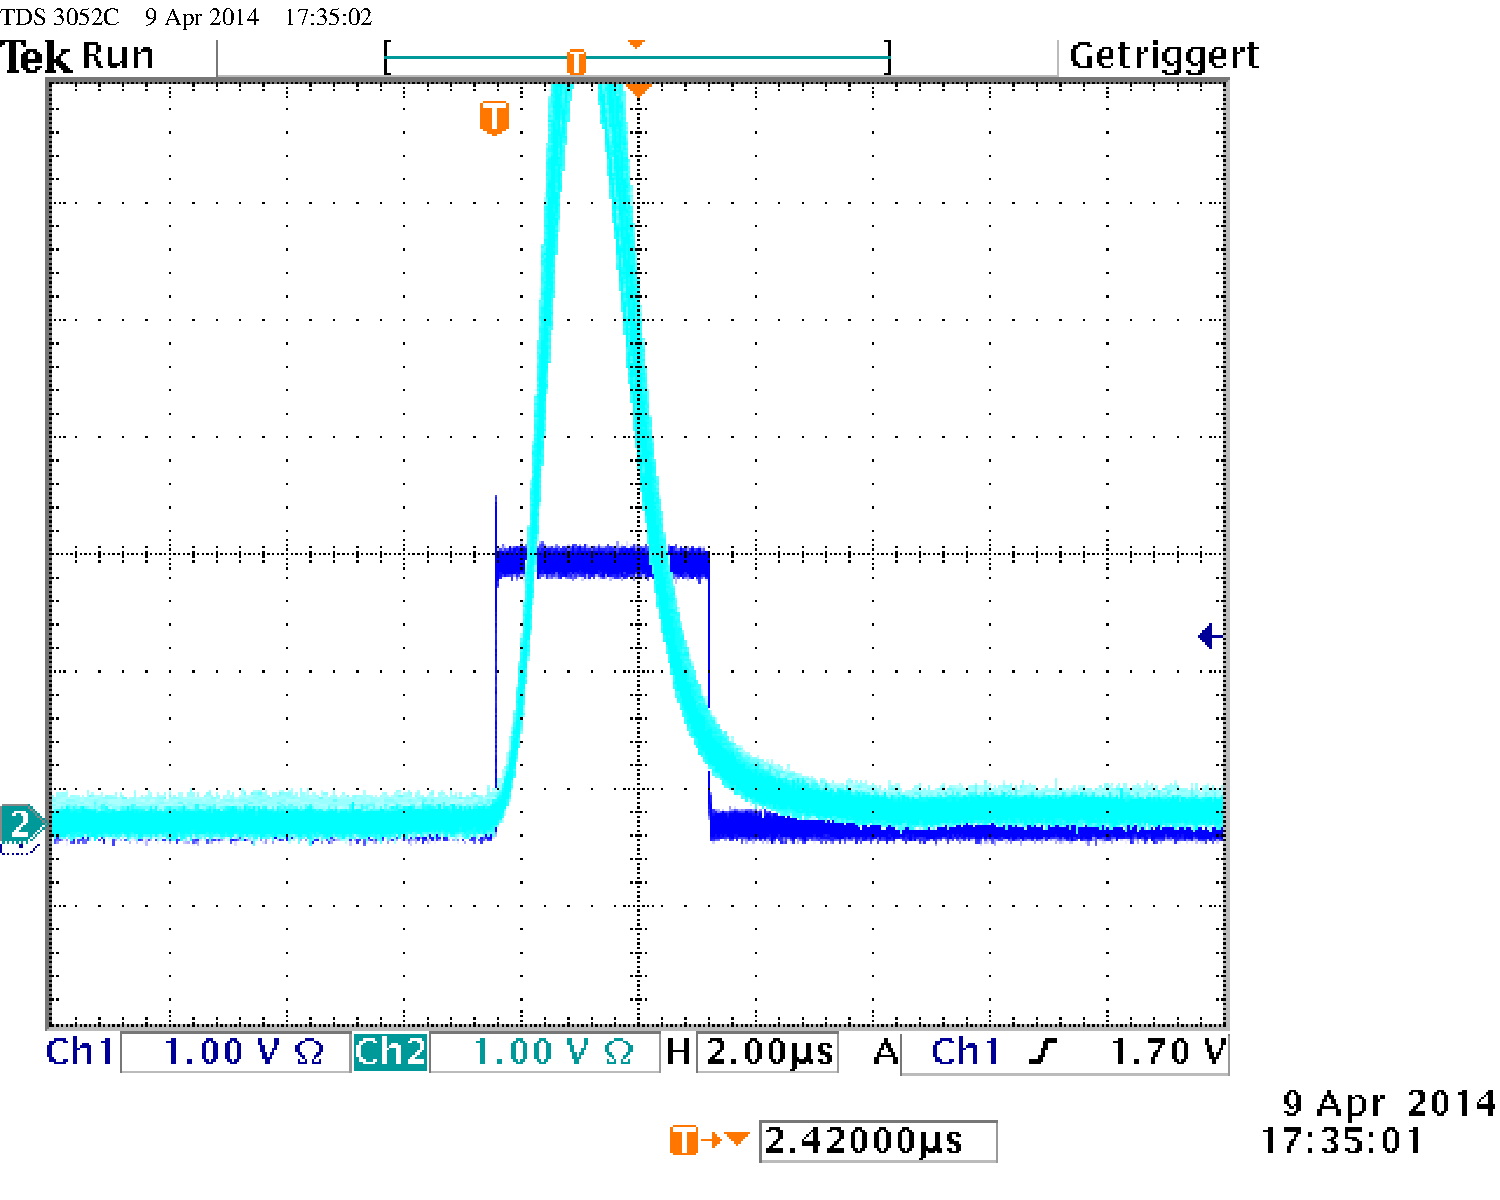
\includegraphics[width=0.49\linewidth]{../Daten/2014-04-09_17-35-east.pdf}
    \hfill
    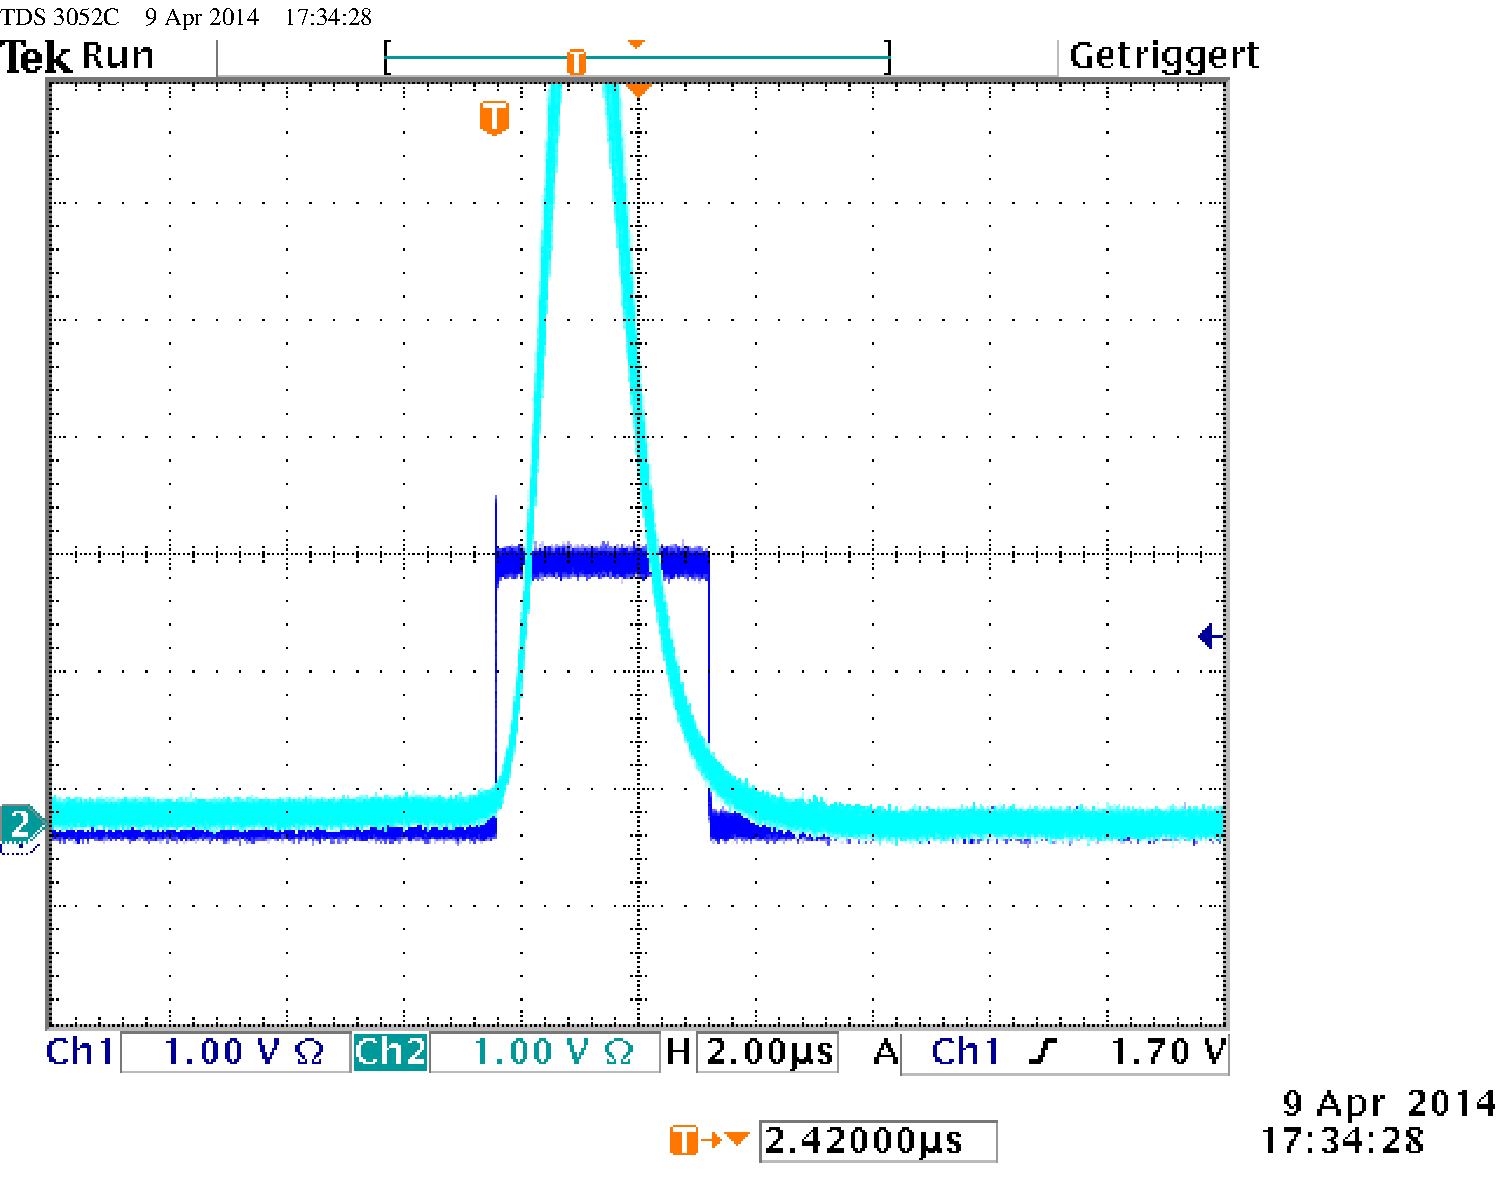
\includegraphics[width=0.49\linewidth]{../Daten/2014-04-09_17-34-east.pdf}
    \caption{%
        Durch den auf die \SI{511}{\kilo\electronvolt}-Linie eingestellten SCA
        erhalten wir im Oszilloskop mit dem Trigger auf dem zweiten Kanal nur
        noch eine Pulshöhe.
    }
    \label{fig:eine_pulshoehe}
\end{figure}

\subsection{Slow-Koinzidenz herstellen}

Wir schließen beide SCA gleichzeitig an das Oszilloskop an. Der rechte Detektor
ist auf Kanal 1 (Bildzeit 17:38), siehe Abbildung~\ref{fig:beide_sca}. Die
beiden Signale liegen ausreichend genau aufeinander, es herrscht Koinzidenz.

\begin{figure}[htbp]
    \centering
    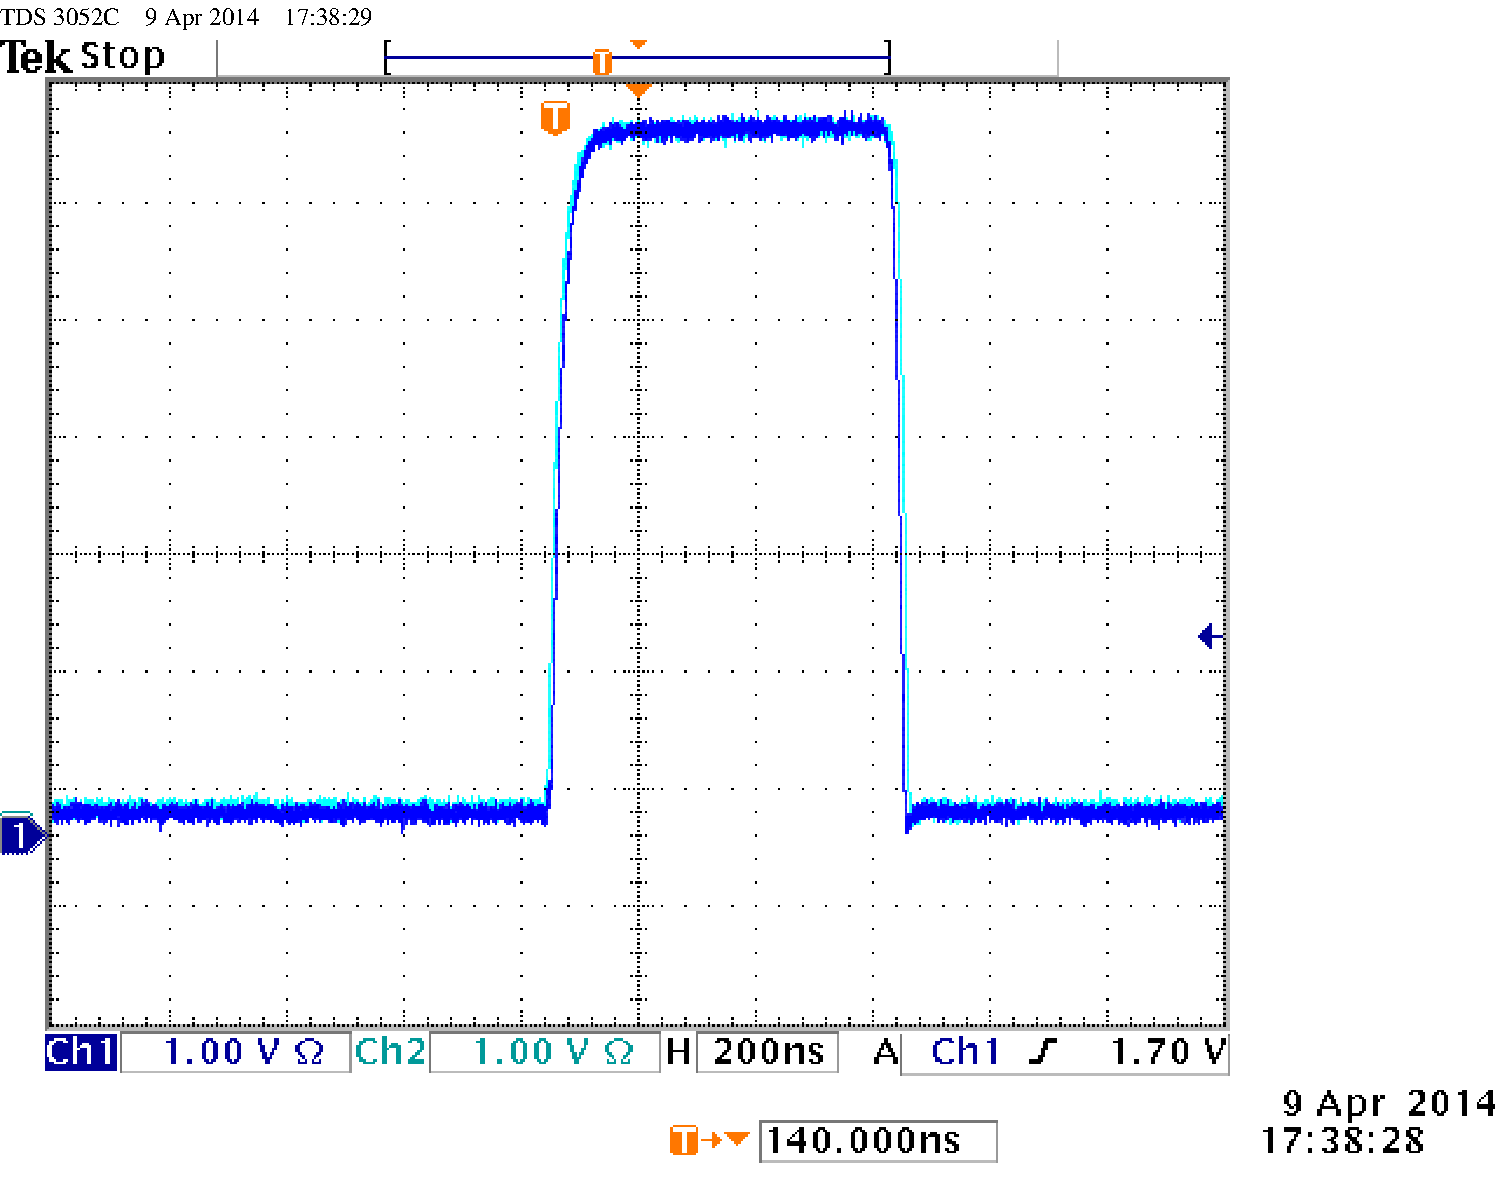
\includegraphics[width=0.49\linewidth]{../Daten/2014-04-09_17-38-east.pdf}
    \hfill
    \caption{%
        Die Signale von beiden SCA gleichzeitig auf dem Oszilloskop.
    }
    \label{fig:beide_sca}
\end{figure}

\section{Fast-Konzidenzkreis einstellen}

Wir beginnen mit der Einstellung des Fast-Kreises am rechten Detektor. Wir
betrachten das Slow-Signal nach dem Vorverstärker und das Fast-Signal zusammen
auf dem Oszilloskop (Bildzeit 09:27). Das gleiche wiederholen wir für den
linken Detektor (Bildzeit 09:29).

Dann schließen wir den linken Hauptverstärker über das Delay an das Oszilloskop
an. Das Signal des rechten Fast-Ausgangs wird an das CFD und dessen negativer
Ausgang an das Oszilloskop angeschlossen, siehe
Abbildung~\ref{fig:aufbau:fast1}. Wir nehmen ein Bild mit Baseline auf (Bild
09:50). Nun erhöhen wir die Schwelle am CFD auf \num{0.4}, so dass die Baseline
verschwindet (Bild 09:51). Dies wiederholen wir für den rechten Zweig. Beim
rechte CFD hat schon bei unterster Schwelleneinstellung keine Baseline (Bild
10:17). Daher werden wir den linken CFD als Stop-Signal zu benutzen, damit wir
die \SI{81}{\kilo\electronvolt}-Linie nicht abschneiden.

\begin{figure}[htbp]
    \centering
    \begin{tikzpicture}
        \node[device] (na) {$^{22}\mathrm{Na}$};
        \node[device] (pm) [right=of na] {Photomultiplier};
        \node[device] (amp) [right=of pm] {Verstärker};
        \node[device] (delay) [right=of amp] {Delay};
        \node[device] (cfd) [below=of pm] {CFD};
        \node[monitor] (oszi) [below=of delay] {Oszilloskop};

        % Teilchenaustausch
        \begin{scope}[->, dotted, thick]
            \draw (na) -- (pm);
        \end{scope}

        % Analogsignal
        \begin{scope}[->]
            \draw (pm) -- (amp);
            \draw (amp) -- (delay);
            \draw (delay) -- (oszi);
            \draw (pm) -- (cfd);
        \end{scope}

        % Digitalsignal
        \begin{scope}[->, dashdotted]
            \draw (cfd) -- (oszi);
        \end{scope}
    \end{tikzpicture}
    \caption{%
    }
    \label{fig:aufbau:fast1}
\end{figure}

Wir schließen den CFD, den wir für das Stop-Signal nutzen wollen, noch an ein
Delay an. Delay und den Start-CFD geben wir auf das Oszilloskop (Bildzeit
10:27), Abbildung~\ref{fig:aufbau:fast2}. Danach geben wir beide CFD Signale (mit Delay) auf das TAC.

\begin{figure}[htbp]
    \centering
    \begin{tikzpicture}
        \node[device] (na) {$^{22}\mathrm{Na}$};
        \node[device] (pm1) [above=of na] {Photomultiplier};
        \node[device] (pm2) [below=of na] {Photomultiplier};
        \node[device] (cfd1) [right=of pm1] {CFD};
        \node[device] (cfd2) [right=of pm2] {CFD};
        \node[device] (delay) [right=of cfd2] {Delay};
        \node[monitor] (oszi) [above=of delay] {Oszilloskop};

        % Teilchenaustausch
        \begin{scope}[->, dotted, thick]
            \draw (na) -- (pm1);
            \draw (na) -- (pm2);
        \end{scope}

        % Analogsignal
        \begin{scope}[->]
            \draw (pm1) -- (cfd1);
            \draw (pm2) -- (cfd2);
        \end{scope}

        % Digitalsignal
        \begin{scope}[->, dashdotted]
            \draw (cfd1) -- (oszi);
            \draw (cfd2) -- (delay);
            \draw (delay) -- (oszi);
        \end{scope}
    \end{tikzpicture}
    \caption{%
    }
    \label{fig:aufbau:fast2}
\end{figure}

\begin{figure}[htbp]
    \centering
    \begin{tikzpicture}
        \node[device] (na) {$^{22}\mathrm{Na}$};
        \node[device] (pm1) [above=of na] {Photomultiplier};
        \node[device] (pm2) [below=of na] {Photomultiplier};
        \node[device] (cfd1) [right=of pm1] {CFD};
        \node[device] (cfd2) [right=of pm2] {CFD};
        \node[device] (delay) [right=of cfd2] {Delay};
        \node[device] (tac) [above=of delay] {TAC};
        \node[monitor] (oszi) [right=of tac] {Oszilloskop};

        % Teilchenaustausch
        \begin{scope}[->, dotted, thick]
            \draw (na) -- (pm1);
            \draw (na) -- (pm2);
        \end{scope}

        % Analogsignal
        \begin{scope}[->]
            \draw (pm1) -- (cfd1);
            \draw (pm2) -- (cfd2);
            \draw (tac) -- (oszi);
        \end{scope}

        % Digitalsignal
        \begin{scope}[->, dashdotted]
            \draw (cfd1) -- (tac);
            \draw (cfd2) -- (delay);
            \draw (delay) -- (tac);
        \end{scope}
    \end{tikzpicture}
    \caption{%
    }
    \label{fig:aufbau:fast2}
\end{figure}

\section{Zeiteichung des TAC}

Wir prüfen erneut die Slow-Koinzidenz (Bildzeit 10:39). Dann schließen wir GDG
an das Oszilloskop an, das TAC an den zweiten Kanal (Bildzeit 10:49). Zuletzt
schließen wir den GDG und das TAC an das MCA an und nehmen Promptkurven auf.

\section{Messung der Lebensdauer}

Wir tauschen Natrium gegen Barium aus. Rechtes Slow-Signal mit Splitter auf SCA
und dan GDG, das andere über Delay und beide auf das Oszilloskop. Signale
übereinander gelegt (Bildzeit rechts 12:28, links 12:27). Dann ein Spektrum
aufgenommen (009). Dann SCA Fenster so eingestellt, dass die nur 350 Linie drin
ist (010).

Mit dem linken Slow-Zweig gehen wir gleich vor, wir nehmen ein Spektrum (011). SCA Fenster (012).

Die Slow-Koinzidenz überprüfen wir mit dem Oszilloskop (Bildzeit 13:10).

Wir betrachten rechte Slow-Signal und Start-CFD-Signal auf dem Oszilloskop
(Bildzeit 13:18). Die Schwelle des CFD stellen wir auf das Minimum. Dann
wechseln wir auf den Stop-Zweig (links) und betrachten zuerst ohne Schwelle
(Bildzeit 13:21). Anschließend stellen wir die Schwelle ein (Bildzeit 13:23).

Wir überprüfen nun die Fast-Koinzidenz, indem wir Start- und Stop-Signal am
Oszilloskop betrachten.

CFD Stelle nach dem Skript, in dem wir das Slow-Signal und negatives Stop-CFD Signal
auf das MCA geben. Die Schwelle des Stop-CFD stellen wir so, dass die
für die Röntgenlinie keine Ereignisse mehr registriert werden (013).

\hrule

\parencite{Bieling/K125}

\begin{tikzpicture}[
        device/.style={
            rectangle,
            minimum size=6mm,
            draw=black
        },
        amp/.style={
            isosceles triangle,
            minimum size=6mm,
            draw=black
        },
    ]

    \node[device] (koinzidenz) at (9.5, -1) {Koinzidenzeinheit};
    \node[device] (gdg) [right=of koinzidenz] {GDG};
    \node[device] (mca) [right=of gdg] {MCA};
    \node[device] (pc) [below=of mca] {PC};

    \begin{scope}[start chain, node distance=5mm, every node/.style={join}, every join/.style={->}]
        \node[device, on chain] (22Na) at (0, 0) {$^{22}\mathrm{Na}$};

        \begin{scope}[start branch=22Na]
            \node[device, on chain=going below, node distance=1.5cm] (Szintillator1) {Szintillator};
            \node[device, on chain] (PM2) {PM};
            \node[amp, on chain] (PA2) {Pre Amp};

            \begin{scope}[start branch=PA2]
                \node[amp, on chain=going below right] (amp2) {Amp};
                \node[device, on chain] (splitter2) {Splitter};
                \begin{scope}[start branch=splitter2]
                    \node[device, on chain=going below right] (delay2) {Delay Amp};
                \end{scope}
                \begin{scope}[start branch=splitter2]
                    \node[device, on chain=going above right] (sca2) {SCA};
                \end{scope}

            \end{scope}
            \node[device, on chain=going above right] (cfd2) {CFD};
            \node[device, on chain] (cfddelay) {Delay};
        \end{scope}

        \node[device, on chain=going above, node distance=1.5cm] (Szintillator1) {Szintillator};
        \node[device, on chain] (PM1) {PM};
        \node[amp, on chain] (PA1) {Pre Amp};

        \begin{scope}[start branch=PA1]
            \node[amp, on chain=going above right] (amp1) {Amp};
            \node[device, on chain] (splitter1) {Splitter};
            \begin{scope}[start branch=splitter1]
                \node[device, on chain=going above right] (delay1) {Delay Amp};
            \end{scope}
            \begin{scope}[start branch=splitter1]
                \node[device, on chain=going below right] (sca1) {SCA};
            \end{scope}
        \end{scope}

        \node[device, on chain=going below right] (cfd1) {CFD};
        \node[device, on chain=going right, node distance=2cm, join=with cfddelay] (tac) {TAC};
        \node[device, on chain=going right, node distance=2cm] (delay3) {Delay Amp};

    \end{scope}

    \begin{scope}[->]
        \draw (delay3) -- (mca);
        \draw (mca) -- (pc);

        \begin{scope}[dashdotted]
            \draw (gdg) -- (mca);
            \draw (sca1) -- (koinzidenz);
            \draw (koinzidenz) -- (gdg);
            \draw (sca2) -- (koinzidenz);
        \end{scope}
    \end{scope}
\end{tikzpicture}

\parencite{Leo/Techniques_Nuclear_Experiments}


\chapter{Auswertung}

\chapter{Ergebnis}

\IfFileExists{\bibliographyfile}{
    \printbibliography
}{}

\end{document}

% vim: spell spelllang=de tw=79
